\documentclass[a5paper,oneside,openany,headings=small]{scrbook}
\usepackage[utf8]{inputenc}
%\usepackage[latin1]{inputenc}
\usepackage[T1]{fontenc} 
\usepackage[top = 2cm, left = 2cm, right = 2cm, bottom = 3cm]{geometry}
\usepackage{ngerman,graphicx,color,cancel}
\usepackage{amsmath}
\usepackage{amssymb}
\usepackage{graphicx}
\usepackage{listings} %code einbinden
\usepackage{subfig}
\usepackage[subfigure]{tocloft}
\usepackage{float}
\usepackage{pdfpages}
\usepackage[automark]{scrlayer-scrpage}
\usepackage{color}
\usepackage{xcolor}
\usepackage{sectsty}
\usepackage{array}\setlength{\extrarowheight}{2pt}
\usepackage{longtable}
\usepackage{xcolor}
\usepackage{array}
\usepackage{hyperref}

\definecolor{forestgreen}{rgb}{0.0,0.4,0.0}

\definecolor{myyellow}{HTML}{d4d400}

\definecolor{Purple}{rgb}{128, 0, 128}

\newcommand{\MyHookSign}{\hbox{\ensuremath\hookleftarrow}}




\automark[chapter]{chapter}
%\automark[chapter]{section}

%\deftripstyle{Flughandbuch}[0pt][1pt]{}{}{\pagemark}{Flughandbuch B12}{}{Akaflieg Berlin e.V.}
\deftripstyle{Flughandbuch}[.5pt][.5pt]{\pagemark}{}{\headmark}{Flug- und Betriebshandbuch B13}{}{05.2013}
\pagestyle{Flughandbuch}
\renewcommand*\chapterpagestyle{Flughandbuch}

\begin{document}
\begin{titlepage}
\thispagestyle{empty}
\vspace{2cm}
\begin{center}
\textbf{Flug- und Betriebshandbuch für den Motorsegler}
\end{center}
\begin{center}
\huge{\textbf{B13}}\\
\end{center}
\begin{center}
Ausgabe 05.2013
\end{center}
\begin{center}
\begin{tabular}{|c|}
\hline
Dieses Handbuch ist stets an Bord mitzuführen\\
\hline

\end{tabular}
\end{center}




\begin{figure}[h]
\begin{center}
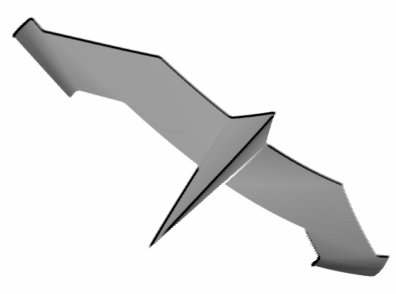
\includegraphics[width=0.3\textwidth]{charlotte.png}
\end{center}
\end{figure}

\begin{tabular}{l l}
Werknummer & 001\\
 & \\
Kennzeichen & D-KILU\\
 & \\

  Hersteller & Akademische Fliegergruppe Berlin e.V.\\
  & Straße des 17. Juni 135\\
  & 10623 Berlin\\

\end{tabular}\\  
\newline
Die mit "`LBA-anerkannt"' gekennzeichneten Blätter sind anerkannt vom Luftfahrtbundesamt, Bundesrepublik Deutschland.\\
Diese Blätter sind auf weißem bzw. rotem Papier gedruckt. Rot kennzeichnet die Notverfahren. Wichtige Stellen sind farblich hervorgehoben.\\
\newline
Unterschrift:\\
\newline
Stempel:\\
\newline
Datum der Anerkennung:
\end{titlepage}
\newpage
\mbox{} \thispagestyle{empty}
\newpage
\pagenumbering{Roman}
%\newpage
\setlength\parindent{0pt}
\tableofcontents
\newpage
\thispagestyle{empty}
\pagenumbering{arabic}
\chapter{Allgemeines}
%\addcontentsline{toc}{section}{Allgemeines}
%\setcounter{section}{1}
%\setcounter{equation}{0}
\section{Einführung}
Das vorliegende Flughandbuch wurde erstellt, um Piloten und Ausbildern alle notwendigen Informationen für einen sicheren, zweckmäßigen und leistungsoptimierten Betrieb des Motorseglers B13 zu geben.\\
\newline
Das Handbuch enthält zunächst alle Daten die dem Piloten aufgrund der Bauvorschrift JAR-22 zur Verfügung stehen müssen. Es enthält darüber hinaus jedoch eine Reihe weiterer Daten und Betriebshinweise, die aus Herstellersicht für den Piloten von Nutzen sein können.

\section{Zulassungsbasis}
Der Motorsegler B13 wird im Rahmen einer "`Vorläufigen Verkehrszulassung"' betrieben. Die Zulassungsbasis stellt die JAR-22 vom 15. März 1982.\\
\newline
Lufttüchtigkeitsgruppe: Utility
\newpage
\section{Hinweisstellen}
Für die Flugsicherheit oder Handhabung besonders bedeutsame Handbuchaussagen sind durch Voranstellung eines der nachfolgenden Begriffe besonders hervorgehoben:\\
\newline
\newline
\begin{color}{red}
\large{\underline{Warnung}}\\
bedeutet, dass die Nichteinhaltung einer entsprechend gekennzeichneten Verfahrensvorschrift zu einer unmittelbaren oder erheblichen Beeinträchtigung der Flugsicherheit führt.
\end{color}\\
\newline
\begin{color}{forestgreen}
\large{\underline{Wichtiger Hinweis}}\\
bedeutet, dass die Nichteinhaltung einer entsprechend gekennzeichneten Verfahrensvorschrift zu einer geringfügigen oder einer mehr oder weniger langfristig eintretenden Beeinträchtigung der Flugsicherheit führt.
\end{color}\\
\newline
\begin{color}{blue}
\large{\underline{Anmerkung}}\\
soll die Aufmerksamkeit auf Sachverhalte lenken, die nicht unmittelbar mit der Sicherheit zusammenhängen, die aber wichtig oder ungewöhnlich sind.
\end{color}

\section{Beschreibung und technische Daten}
Die B13 ist ein doppelsitziger Motorsegler mit einem gedämpften T-Leitwerk, 4-teiligen Tragflächen, nebeneinander angeordneten Sitzen, Schempp-Hirth Oberseiten-Bremsklappen und einem gefederten Hauptfahrwerk.\\
\newline
Die B13 wurde für wissenschaftliche Zwecke und für den Leistungsflug entworfen.
\newpage
\textbf{Technische Daten}\\

\begin{longtable}{l l l}
Besatzung & & 1+1\\
 & & \\
 Tragflügel & & \\
  & Spannweite & $23,20m$\\
  & Fläche & $18,95m^2$\\
  & Streckung & $28,4$ \\
  & Ersatzflügeltiefe & $873mm$ \\
  & Einstellwinkel & $0^{\circ}$ \\
  & Pfeilung zur $25\%$-Linie & $-0,3^{\circ}$ \\
  & V-Stellung & $1^{\circ}$\\
  & Verwindung & $0^{\circ}$\\
  & Profil & HQ 41/14,35\\
  & Klappentiefe & $17,5\%$ \\
  & & \\
 Rumpf & & \\
 & Länge & $8,55m$\\
 & Breite & $1,28m$\\
 & Höhe & $0,90m$ \\
 & & \\
 Höhenleitwerk & & \\
 & Spannweite & $3,10m$\\
 & Fläche & $1,457m^2$\\
 & Profil & FX 71-L-150/25 \\
 & & \\
 Seitenleitwerk & & \\
 & Höhe & $1,70m$ \\
 & Fläche & $1,71m^2$\\
 & Profil & FX 71-L-150/30\\
 & & \\
 Bremsklappen & & \\
 & Spannweite & $1,50m$\\
 & Höhe & $158mm$ \\
 & Fläche & $0,442m^2$\\
 & & \\
 Fahrwerk & & \\
 & Hauptrad, einziehbar & $380$x$150, 3-3,5Bar$\\
 & Heckrad, fest & $210$x$65, 2,5-2,8Bar$\\
 & Radstand & $5,60m$\\
 & & \\
 Triebwerk & & nicht eingebaut\\
 & & \\
 Massen & & \\
 & Leermasse & s. Wägebericht\\
 & Höchstmasse & $820kg$\\
 & Flächenbelastung min/max & $34,7\frac{kg}{m^2}$/$43,3\frac{kg}{m^2}$\\
 & & \\
 Flugleistungen & bei Flugmasse $765kg$ & \\
 & beste Gleitzahl (WK +1) & $45,4 (95\frac{km}{h})$ \\
 & geringstes Sinken (WK +1) & $0,56\frac{m}{s} (90\frac{km}{h})$

\end{longtable}

\section{Dreiseitenansicht}
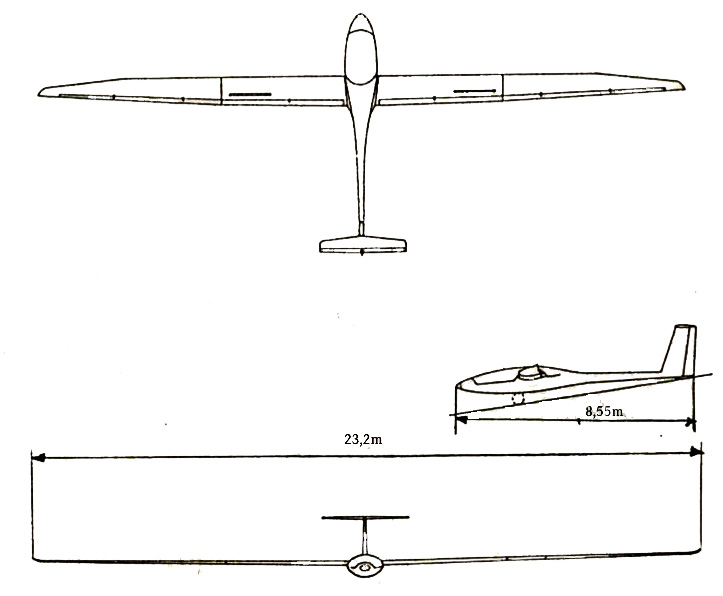
\includegraphics[width=\textwidth]{3seiten.jpg}
\deftripstyle{Flughandbuch}[.5pt][.5pt]{\pagemark}{}{\headmark}{Flug- und Betriebshandbuch B13}{}{LBA-anerkannt 06.2022}
\pagestyle{Flughandbuch}
\renewcommand*\chapterpagestyle{Flughandbuch}


\chapter{ Betriebsgrenzen}

\section{Einführung}
Der vorliegende Abschnitt beinhaltet Betriebsgrenzen, Instrumentenmarkierungen und Hinweisschilder, die für den sicheren Betrieb der B13 notwendig sind. 

\section{Fluggeschwindigkeiten}

Die Fluggeschwindigkeitsgrenzen und ihre Bedeutung für den Betrieb sind nachfolgend aufgeführt:

\begin{longtable}{|p{0.11\textwidth}|m{0.25\textwidth}|p{0.15\textwidth}|m{0.35\textwidth}|llll}
\hline
& Geschwindigkeit & IAS [$\unit{\frac{km}{h}}$] & Anmerkungen \\
\hline
$V_{NE}$ & Zulässige Höchst"-ge"-schwin"-digkeit bei ruhigem Wetter & $220$ & Diese Geschwindigkeit darf nicht überschritten werden und der Ruderausschlag darf nicht mehr als $\frac{1}{3}$ betragen\\
\hline
$V_{RA}$ & Zulässige Höchstge"-schwindigkeit in starker Turbulenz & $180$ & Diese Geschwindigkeit darf bei starker Turbulenz nicht überschritten werden. (Starke Turbulenz herrscht vor in Leewellen-Rotoren, Gewitterwolken, usw.) \\
\hline
$V_A$ & Manöver"-geschwindigkeit & $180$ & Oberhalb dieser Geschwindigkeit dürfen keine vollen oder abrupten Ruderausschläge ausgeführt werden, da die Flugzeugstruktur dabei überlastet werden könnte.\\
\hline
$V_{FE}$ & Zulässige Höchstges"-chwindigkeit für das Betätigen der Flügelklappen
&   & Diese Geschwindigkeit darf bei der angegebenen Flügelklappenstellung nicht überschritten werden.\\
& +2, +1 & 180 & \\
& Landestellung L & 130 & \\
\hline
$V_W$ & Zulässige Höchstge"-schwindigkeit für den Windenschlepp & $120$ & Diese Geschwindigkeit darf während des Winden- oder Kraftfahrzeugschlepps nicht überschritten werden.\\
\hline
$V_T$ & Zulässige Höchstge"-schwindigkeit für den Flugzeugschlepp & $160$ & Diese Geschwindigkeit darf während des Flugzeugschlepps nicht überschritten werden.\\
\hline
$V_{LO}$ & Zulässige Höchstge"-schwindigkeit zum Betätigen des Fahrwerks & $160$ & Über dieser Geschwindigkeit darf das Fahrwerk nicht ein- oder ausgefahren werden.\\
\hline
$V_{PO}$ & Zulässige Geschwindigkeit mit drehendem Propeller & 160 (Vorläufig) & Diese Geschwindigkeit darf bei drehendem Propeller nicht überschritten werden. (Unabhängig von der eingestellten Motorleistung)\\
\hline
$V_{PO,min}$ & Zulässige Mindestge"-schwindigkeit für den Start des Triebwerks & 80 (Vorläufig) & Unterhalb dieser Geschwindigkeit darf der Motor nicht gestartet werden\\
\hline
$V_{PO,max}$ & Zulässige Maximalge"-schwindigkeit für den Start des Triebwerks & 135 (Vorläufig) & Oberhalb dieser Geschwindigkeit darf der Motor nicht gestartet oder abgestellt werden\\
\hline
\end{longtable}

\begin{color}{red}
\large{\underline{Warnung}}\\
Wählen Sie die richtige Geschwindigkeit zum Starten/Stoppen des Motors: \\
Stellen Sie sicher, dass Ihre gewählte Start- und Stopp- Geschwindigkeit des Motor mindestens $\unit[8-10]{km/h}$ über der Überziehgeschwindigkeit der gewählten Flugkonfiguration liegt.
\end{color}\\
\newpage
\section{Anzeigefehler in der Fahrtmesseranlage}
Die folgenden Angaben sind als die berichtigten Fluggeschwindigkeiten $v_{CAS}$ über der Differenz zur angezeigten Fluggeschwindigkeit $v_{IAS}$ dargestellt. Es wurde dabei ein Instrumentenfehler gleich Null angenommen. Die Darstellung erfasst weiterhin alle Flügelklappen"-stellungen und deckt den entsprechenden Geschwindigkeitsbereich ab.\\
\newline
Die Druckentnahme erfolgt durch eine Kombidüse an der Nase vom Seitenleitwerk.\\
\newline
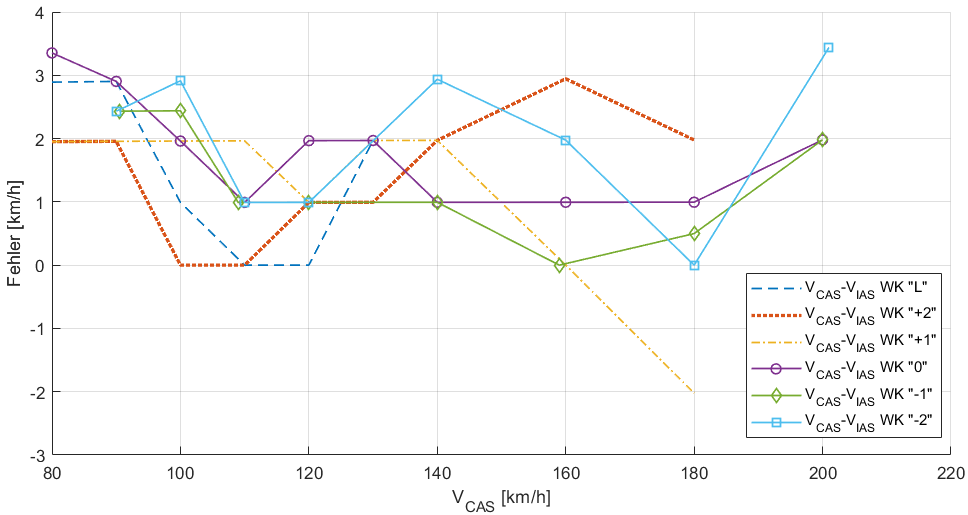
\includegraphics[width=\textwidth]{Fahrtmesserkalibrierung2.png}
\newline
Der Fehler der Fahrtmesseranlage beträgt nicht mehr als $8 \frac{km}{h}$ bzw. $5\%$ und erfüllt damit die Anforderungen der JAR 22 (siehe JAR 22.1323).

\section{Überziehgeschwindigkeiten}

Die folgenden Überziehgeschwindigkeiten \textbf{ohne Motor} wurden bei einem Abfluggewicht von $\unit[820]{kg}$ und vorderster Schwerpunktlage ermittelt:\\

\textbf{Ohne Motor:}

\begin{longtable}{l l l}
WK $-2$ & & \\
& Geradeaus: & $\unit[78]{\frac{km}{h}}$\\
& $5^{\circ}$ schiebend: & $\unit[78]{\frac{km}{h}}$\\
& $45^{\circ}$-Kurve: & $\unit[95]{\frac{km}{h}}$\\
%& &  \\
\hline
& &  \\
WK $-1$ & & \\
& Geradeaus: & $\unit[79]{\frac{km}{h}}$\\
& $5^{\circ}$ schiebend: & $\unit[79]{\frac{km}{h}}$\\
& $45^{\circ}$-Kurve: & $\unit[88]{\frac{km}{h}}$\\
%& &  \\
\hline
& &  \\
WK $0$ & & \\
& Geradeaus: & $\unit[79]{\frac{km}{h}}$\\
& $5^{\circ}$ schiebend: & $\unit[79]{\frac{km}{h}}$\\
& $45^{\circ}$-Kurve: & $\unit[90]{\frac{km}{h}}$\\
%& &  \\
\hline
& &  \\
WK $+1$ & & \\
& Geradeaus: & $\unit[77]{\frac{km}{h}}$\\
& $5^{\circ}$ schiebend: & $\unit[77]{\frac{km}{h}}$\\
& $45^{\circ}$-Kurve: & $\unit[89]{\frac{km}{h}}$\\
%& &  \\
\hline
 & & \\
WK $+2$ & & \\
& Geradeaus: & $\unit[76]{\frac{km}{h}}$\\
& $5^{\circ}$ schiebend: & $\unit[76]{\frac{km}{h}}$\\
& $45^{\circ}$-Kurve: & $\unit[85]{\frac{km}{h}}$\\
%& &  \\
\hline
& &  \\
WK L& & \\
& Geradeaus: & $\unit[75]{\frac{km}{h}}$\\
& $5^{\circ}$ schiebend: & $\unit[75]{\frac{km}{h}}$\\
& $45^{\circ}$-Kurve: & $\unit[88]{\frac{km}{h}}$\\
& geradeaus, Bremsklappe + Fahrwerk aus: & $\unit[78]{\frac{km}{h}}$ \\
\end{longtable}

Die folgenden Überziehgeschwindigkeiten \textbf{mit Motor} wurden bei einem Abfluggewicht von $\unit[850]{kg}$ und vorderster Schwerpunktlage ermittelt:\\

\textbf{Mit Motor im Leerlauf:}
ACHTUNG! Daten noch nicht komplett eingetragen - Stand 2022-07-11
\begin{longtable}{l l l}
WK $-2$ & & \\
& Geradeaus: & $\unit[80]{\frac{km}{h}}$\\
& $5^{\circ}$ schiebend: & $\unit[80]{\frac{km}{h}}$\\
& $45^{\circ}$-Kurve: & $\unit[95]{\frac{km}{h}}$\\
%& &  \\
\hline
& &  \\
WK $-1$ & & \\
& Geradeaus: & $\unit[70]{\frac{km}{h}}$\\
& $5^{\circ}$ schiebend: & $\unit[70]{\frac{km}{h}}$\\
& $45^{\circ}$-Kurve: & $\unit[88]{\frac{km}{h}}$\\
%& &  \\
\hline
& &  \\
WK $0$ & & \\
& Geradeaus: & $\unit[70]{\frac{km}{h}}$\\
& $5^{\circ}$ schiebend: & $\unit[70]{\frac{km}{h}}$\\
& $45^{\circ}$-Kurve: & $\unit[90]{\frac{km}{h}}$\\
%& &  \\
\hline
& &  \\
WK $+1$ & & \\
& Geradeaus: & $\unit[80]{\frac{km}{h}}$\\
& $5^{\circ}$ schiebend: & $\unit[80]{\frac{km}{h}}$\\
& $45^{\circ}$-Kurve: & $\unit[89]{\frac{km}{h}}$\\
%& &  \\
\hline
 & & \\
WK $+2$ & & \\
& Geradeaus: & $\unit[79]{\frac{km}{h}}$\\
& $5^{\circ}$ schiebend: & $\unit[79]{\frac{km}{h}}$\\
& $45^{\circ}$-Kurve: & $\unit[85]{\frac{km}{h}}$\\
%& &  \\
\hline
& &  \\
WK L& & \\
& Geradeaus: & $\unit[70]{\frac{km}{h}}$\\
& $5^{\circ}$ schiebend: & $\unit[70]{\frac{km}{h}}$\\
& $45^{\circ}$-Kurve: & $\unit[88]{\frac{km}{h}}$\\
& geradeaus, Bremsklappe + Fahrwerk aus: & $\unit[78]{\frac{km}{h}}$ \\
\end{longtable}



\section{Fahrtmessermarkierungen}
Die folgende Tabelle nennt die Fahrtmessermarkierungen und die Bedeutung der Farben:\\

\begin{tabular}{|m{1,8cm}|m{1,5cm}|m{6cm}|}
\hline
Markierung & IAS [$\unit{\frac{km}{h}}$] & Bedeutung \\
\hline
Weißer Bogen & $80-180$ & Betriebsbereich für positive Klappenausschläge (Untere Grenze ist die Geschwindigkeit $1,1 \cdot V_{S0}$ bei Höchstmasse in Landekonfiguration. Obere Grenze ist die zulässige Höchstgeschwindigkeit mit positivem Klappenausschlag.)\\
\hline
\begin{color}{forestgreen} Grüner Bogen \end{color} & \begin{color}{forestgreen} $80-180$ \end{color} & \begin{color}{forestgreen} Normaler Betriebsbereich (Untere Grenze ist die Geschwindigkeit $1,1 \cdot V_{S1}$ bei Höchstmasse und vorderster Schwerpunktlage und Flügelklappen in der Neutralstellung; obere Grenze ist die zulässige Höchstgeschwindigkeit in starker Turbulenz) \end{color} \\ 
\hline
\begin{color}{myyellow} Gelber Bogen \end{color} & \begin{color}{myyellow} $180-220$ \end{color} & \begin{color}{myyellow} In diesem Bereich darf bei starker Turbulenz nicht geflogen werden und Manöver dürfen nur mit Vorsicht durchgeführt werden. \end{color}\\
\hline
\begin{color}{red} Roter Strich \end{color} & \begin{color}{red} $220$ \end{color} & \begin{color}{red} Zulässige Höchstgeschwindigkeit für alle Betriebsarten \end{color}\\
\hline
\begin{color}{myyellow} Gelbes Dreieck \end{color} & \begin{color}{myyellow} $95$ \end{color} & \begin{color}{myyellow} Anfluggeschwindigkeit bei Höchstmasse \end{color}\\
\hline
\end{tabular}
\newline

\vspace{0.2cm}
Die B13 hat keine speziellen Fahrmessermarkierungen für den Motorbetrieb.
\newpage
\section{Triebwerk}
\begin{color}{red}
\large{\underline{Warnung}}\\
Die B13 ist nicht für den Eigenstart zugelassen.
\end{color}\\

\subsection{Motor}
\begin{tabular}{p{0.3\textwidth}p{0.6\textwidth}ll}
Motor Hersteller: & Emrax d.o.o.\\
Motor Modell: & Emrax 208 LowVoltage AirCooled\\
\end{tabular}\\

\vspace{0.2cm}
\begin{tabular}{p{0.6\textwidth}p{0.3\textwidth}ll}
Maximale Dauerleistung: & $\unit[22]{kW}$\\
Maximale Leistung für 2 Minuten: & $\unit[30]{kW}$\\
Maximale Drehzahl: & $\unit[5000]{min^{-1}}$
\end{tabular}

\subsection{Propeller}
\begin{tabular}{p{0.3\textwidth}p{0.5\textwidth}ll}
Hersteller: & Akaflieg Berlin e.V. \\
Modell: & B13e Faltpropeller V01 \\
\end{tabular}\\

\vspace{0.2cm}
\begin{tabular}{p{0.6\textwidth}p{0.3\textwidth}ll}
Maximale Dauerdrehzahl: & $\unit[3000]{min^{-1}}$ \\
Kurzzeitige Überdrehzahl: & $\unit[3200]{min^{-1}}$ \\
\end{tabular}

\subsection{Akkupacks}
\begin{tabular}{p{0.4\textwidth}p{0.5\textwidth}ll}
Hersteller: & LZ-Design d.o.o \\
Bezeichnung:& FES GEN2 75Ah \\
\end{tabular}\\

\vspace{0.2cm}
Das Antriebsystem benötigt zwei in Reihe geschaltete Akkupacks. Jedes Akkupack besitzt 14 LiPo Zellen, also insgesamt 28 Zellen.\\

\begin{tabular}{p{0.83\textwidth}p{0.15\textwidth}ll}
Max. zulässige Gesamtspannung beider Akkupacks: & $\unit[118]{V}$ \\
Min. zulässige Gesamtspannung beider Akkupacks: & $\unit[90]{V}$ \\
Nennkapazitat pro Zelle: & $\unit[75]{Ah}$ \\
Energiespeicherkapazitat: & $\unit[7,8]{kWh}$ \\
Maximale Spannung pro Zelle: & $\unit[4,16]{V}$ \\
Nennspannung: & $\unit[3,7]{V}$ \\
Minimale Spannung pro Zelle: & $\unit[3,2]{V}$ \\
\end{tabular}\\

\vspace{0.5cm}
Weitere Informationen über die verwendeten Akkupacks finden Sie im \textbf{FES AKKUPACKHANDBUCH der Firma LZ-Design.}

\section{Markierungen des Triebwerksinstruments}
Das FES Triebwerk besitzt ein FCU Instrument mit einem hochauflösenden
sonnenlichtgeeignetem Farbdisplay. Weitere Informationen über die FCU und Ihre
Bedienung finden Sie im \textbf{FES FCU INSTRUMENTENHANDBUCH!}

\section{Masse (Gewicht)}
\begin{tabular}{l l}
Leermasse & s. Wägebericht\\
Höchstzulässige Abflugmasse & $\unit[820]{kg}$\\
Höchstzulässige Masse nichttragender Teile & $\unit[506]{kg}$ \\
Höchstmasse im Gepäckraum & $\unit[10]{kg}$ \\
\end{tabular}\\

\vspace{0.5cm}
Die Masse der Batterie Packs beträgt insgesamt ca. $\unit[50]{kg}$, der Antriebsstrang mit Motor und Propeller wiegt $\unit[19]{kg}$, der Regler wiegt ca. $\unit[5]{kg}$.\\

\begin{color}{red}
\large{\underline{Warnung}}\\
Die Mindestzuladung ohne Motor und ohne Batterien beträgt ca. $\unit[150]{kg}$!
\end{color}\\


\section{Schwerpunkt}
\begin{tabular}{l l}
Flugzeuglage & Keil $1000:28$ auf der Rumpfoberseite\\
Bezugsebene (BE) & Flügelvorderkante an der Wurzelrippe \\
Größte Vorlage & $\unit[245,3]{mm}$ hinter BE\\
Größte Rücklage & $\unit[428,6]{mm}$ hinter BE\\
\end{tabular}\\

\vspace{0.5cm}
\textbf{Hebelarme}\\
\begin{tabular}{m{6,5cm} m{3cm}}
Piloten & $x_P=\unit[-445]{mm}$\\
Gepäckfach & $x_G=\unit[200]{mm}$\\
\end{tabular}\\

Die Bezugsebene ist die Vorderkante der Wurzelrippe.\\

Die Antriebskomponenten der B13 wurden so positioniert, dass ein großer Zuladungsbereich möglich ist. \\


\begin{color}{red}
\large{\underline{Warnung}}\\
Ein Flug mit ausgebautem Motor ist nur in Verbindung einer neuen Wägung zulässig. Ein Ausbau des Antriebsstrangs erhöht in deutlichem Maße die Mindestzuladung.
\end{color}\\


\begin{color}{red}
\large{\underline{Warnung}}\\
Ein Flug mit ausgebautem Akkupack ist nur in Verbindung einer neuen Wägung zulässig. Ein Ausbau der Akkupacks erhöht in deutlichem Maße die Mindestzuladung.
\end{color}\\

\subsection{Wägebericht}

\begin{tiny}
\begin{tabular}{|m{1,8cm}|m{1,8cm}|m{2cm}|m{1,5cm}|m{1,5cm}|}
\hline
Datum & Leermasse [$\unit{kg}$] & Leermassen- schwerpunkt [$\unit{mm}$]  & Maximale Zuladung [$\unit{kg}$] & Unterschrift\\

\hline
& & & &\\
14.03.12 & 579 & 552,9 & 221 & Hofmann\\
& & & &\\
\hline
& & & &\\
23.02.19 & 655 & 514 & 165 & Döring\\
& & & &\\
\hline
& & & &\\
& & & &\\
& & & &\\
\hline
& & & &\\
& & & &\\
& & & &\\
\hline
& & & &\\
& & & &\\
& & & &\\
\hline

\end{tabular}
\end{tiny}

%\newline
%Weitere Hinweise zur Schwerpunktlage und dem Beladeplan sind dem Kapitel 6 "`Masse und Schwerpunktlage"' zu entnehmen.

\section{Zugelassene Manöver}
Der Motorsegler B13 ist für den normalen Segelflug (Lufttüchtig"-keits"-gruppe "`Utility"') zugelassen.\\
\newline
\begin{color}{red}
\large{\underline{Warnung}}\\
\textbf{Kunstflug ist nicht zulässig}
\end{color}

\section{Manöverlastvielfache}

Folgende Lastvielfache dürfen beim Abfangen nicht überschritten werden.\\
\newline
\begin{tabular}{|l|c|c|}
\hline
& positiv & negativ \\
\hline
Bei Manövergeschwindigkeit $V_A=\unit[160]{\frac{km}{h}}$ & $+5,3$ & $-2,65$\\
\hline
Bei Höchstgeschwindigkeit $V_{NE}=\unit[220]{\frac{km}{h}}$ & $+4,0$ & $-1,5$ \\
\hline
Bei ausgefahrenen Bremsklappen und $V_{NE}$ & $+3,5$ & $0$\\
\hline
\end{tabular}

\section{Flugbesatzung}
Die B13 kann einsitzig oder doppelsitzig geflogen werden. Der verantwortliche Luftfahrzeugführer kann auf der linken oder rechten Seite sitzen. Es wird empfohlen, die Platzrunde und insbesondere bodennahe Kurven (z.B. bei Seilriss) in Richtung des fliegenden Luftfahrzeugführes auszuführen, da ansonsten mit Sichtbeeinträchtigungen gerechnet werden muss.

\section{Betriebsarten}
Mit der B13 dürfen Flüge nach Sichtflugregeln (VFR) bei Tag durchgeführt werden.\\
\newline
\begin{color}{red} \large{\underline{Warnung}}\\
Kunstflug und Wolkenflug sind nicht zulässig
\end{color}\\

\begin{color}{red}
\large{\underline{Warnung}}\\
Flüge bei starkem Regen mit laufendem Motor sind verboten! Es
muss sichergestellt werden, dass die Bestandteile des Elektroantriebes nicht nass werden.
\end{color}\\

\begin{color}{red}
\large{\underline{Warnung}}\\
Eigenstarts mit der B13 sind nicht zulässig.
\end{color}
\newpage
\section{Mindestausrüstung}
Zur Mindestausrüstung für den Normalbetrieb gehören:\\
\begin{itemize}
\item Fahrtmesser (bis $\unit[300]{\frac{km}{h}}$ mit Farbmarkierungen nach Abschnitt 2.3)
\item Höhenmesser
\item Variometer
\item Magnetkompass
\item 2 Anschnallgurte (vierteilig, symmetrisch)
\item Flug- und Betriebshandbuch
\item Daten- und Hinweisschilder
\item 2 automatische oder manuelle Fallschirme
\end{itemize}

\section{Flugzeugschlepp und Windenschlepp}

\textbf{Flugzeugschlepp}\\
Die maximal zulässige Schleppgeschwindigkeit beträgt $V_T=\unit[160]{\frac{km}{h}}$.\\
Es wurden Seillängen zwischen $\unit[30]{m}$ und $\unit[60]{m}$ erprobt.\\
Die Sollbruchstellen des Schleppseils sollten eine Bruchlast von $\unit[1000]{daN}$ (schwarz) erreichen.\\
Für den Flugzeugschlepp wird die Schwerpunktkupplung an der Rumpfunterseite verwendet.\\

\textbf{Windenschlepp}\\
Die maximal zulässige Schleppgeschwindigkeit beträgt $V_W=\unit[120]{\frac{km}{h}}$, $\unit[100]{\frac{km}{h}}$ sollte nicht unterschritten werden.\\
Die Sollbruchstellen des Windenseils sollten eine Bruchlast von $\unit[1000]{daN}$ (schwarz) haben.\\
Für den Windenstart wird die Schwerpunktkupplung an der Rumpfunterseite verwendet.
\newpage

\section{Hinweisschilder für Betriebsgrenzen}

\begin{figure}[h]
\begin{center}
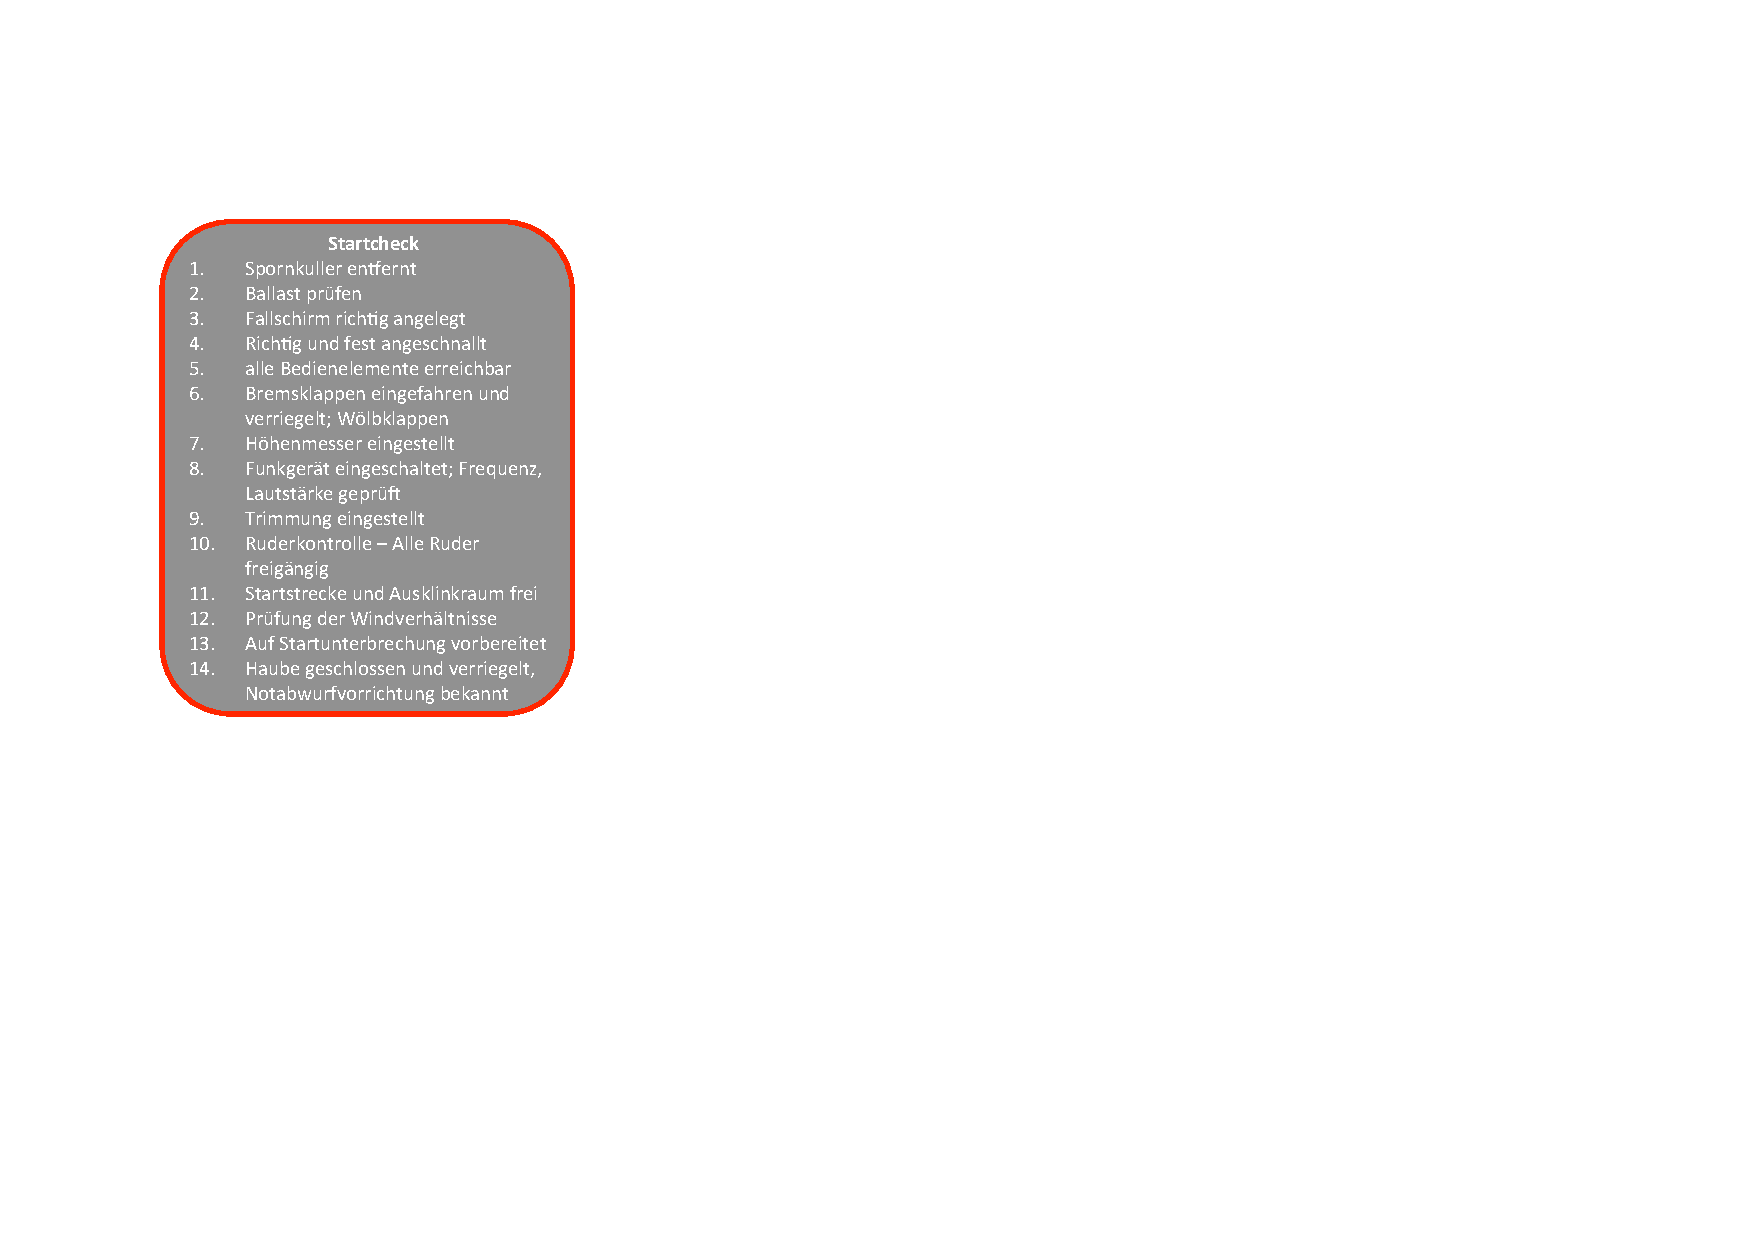
\includegraphics[width=.45\textwidth]{bilder/startcheck.pdf}
\caption*{Startcheck}
\end{center}
\end{figure}

\begin{figure}[h]
\begin{center}
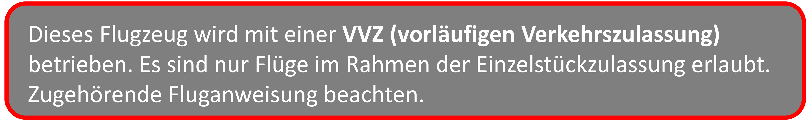
\includegraphics[width=.9\textwidth]{bilder/vvz.pdf}
\caption*{Permit To Fly}
\end{center}
\end{figure}

\begin{figure}[H]
\begin{center}
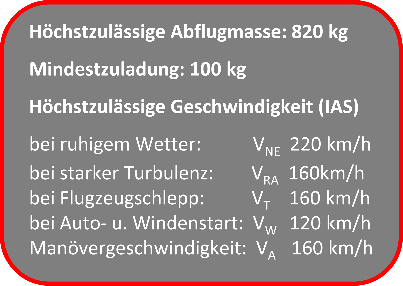
\includegraphics[width=.45\textwidth]{bilder/datenschild.pdf}
\caption*{Datenschild}
\end{center}
\end{figure}

\begin{figure}[H]
\begin{center}

\includegraphics[width=.15\textwidth]{bilder/notabwurf.pdf}\\
\caption*{Haubennotabwurf am Instrumentenbrett}
\end{center}
\end{figure}

\begin{figure}[H]
\begin{center}
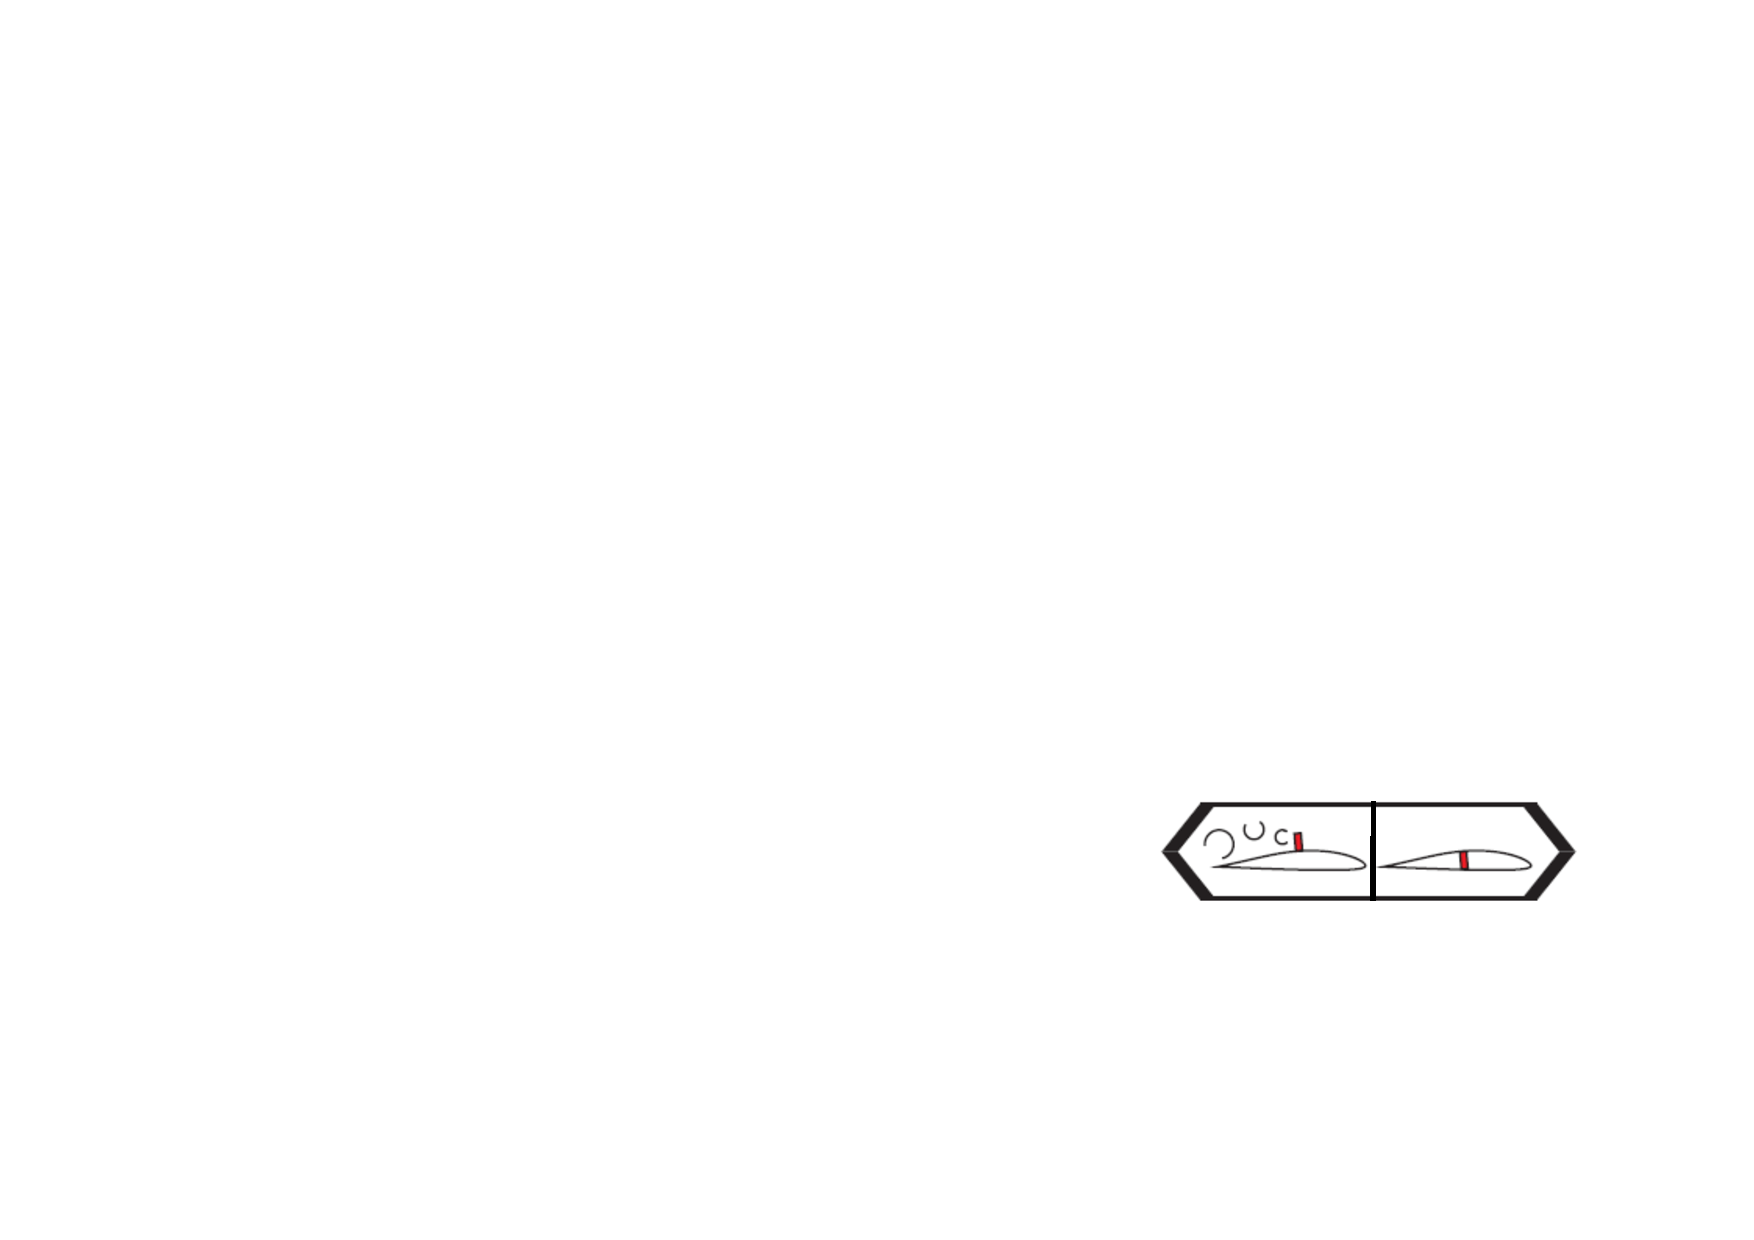
\includegraphics[width=.45\textwidth]{bilder/bk.pdf}
\caption*{Bremsklappen, blauer Griff jeweils links}
\end{center}
\end{figure}


\begin{figure}[H]
\begin{center}
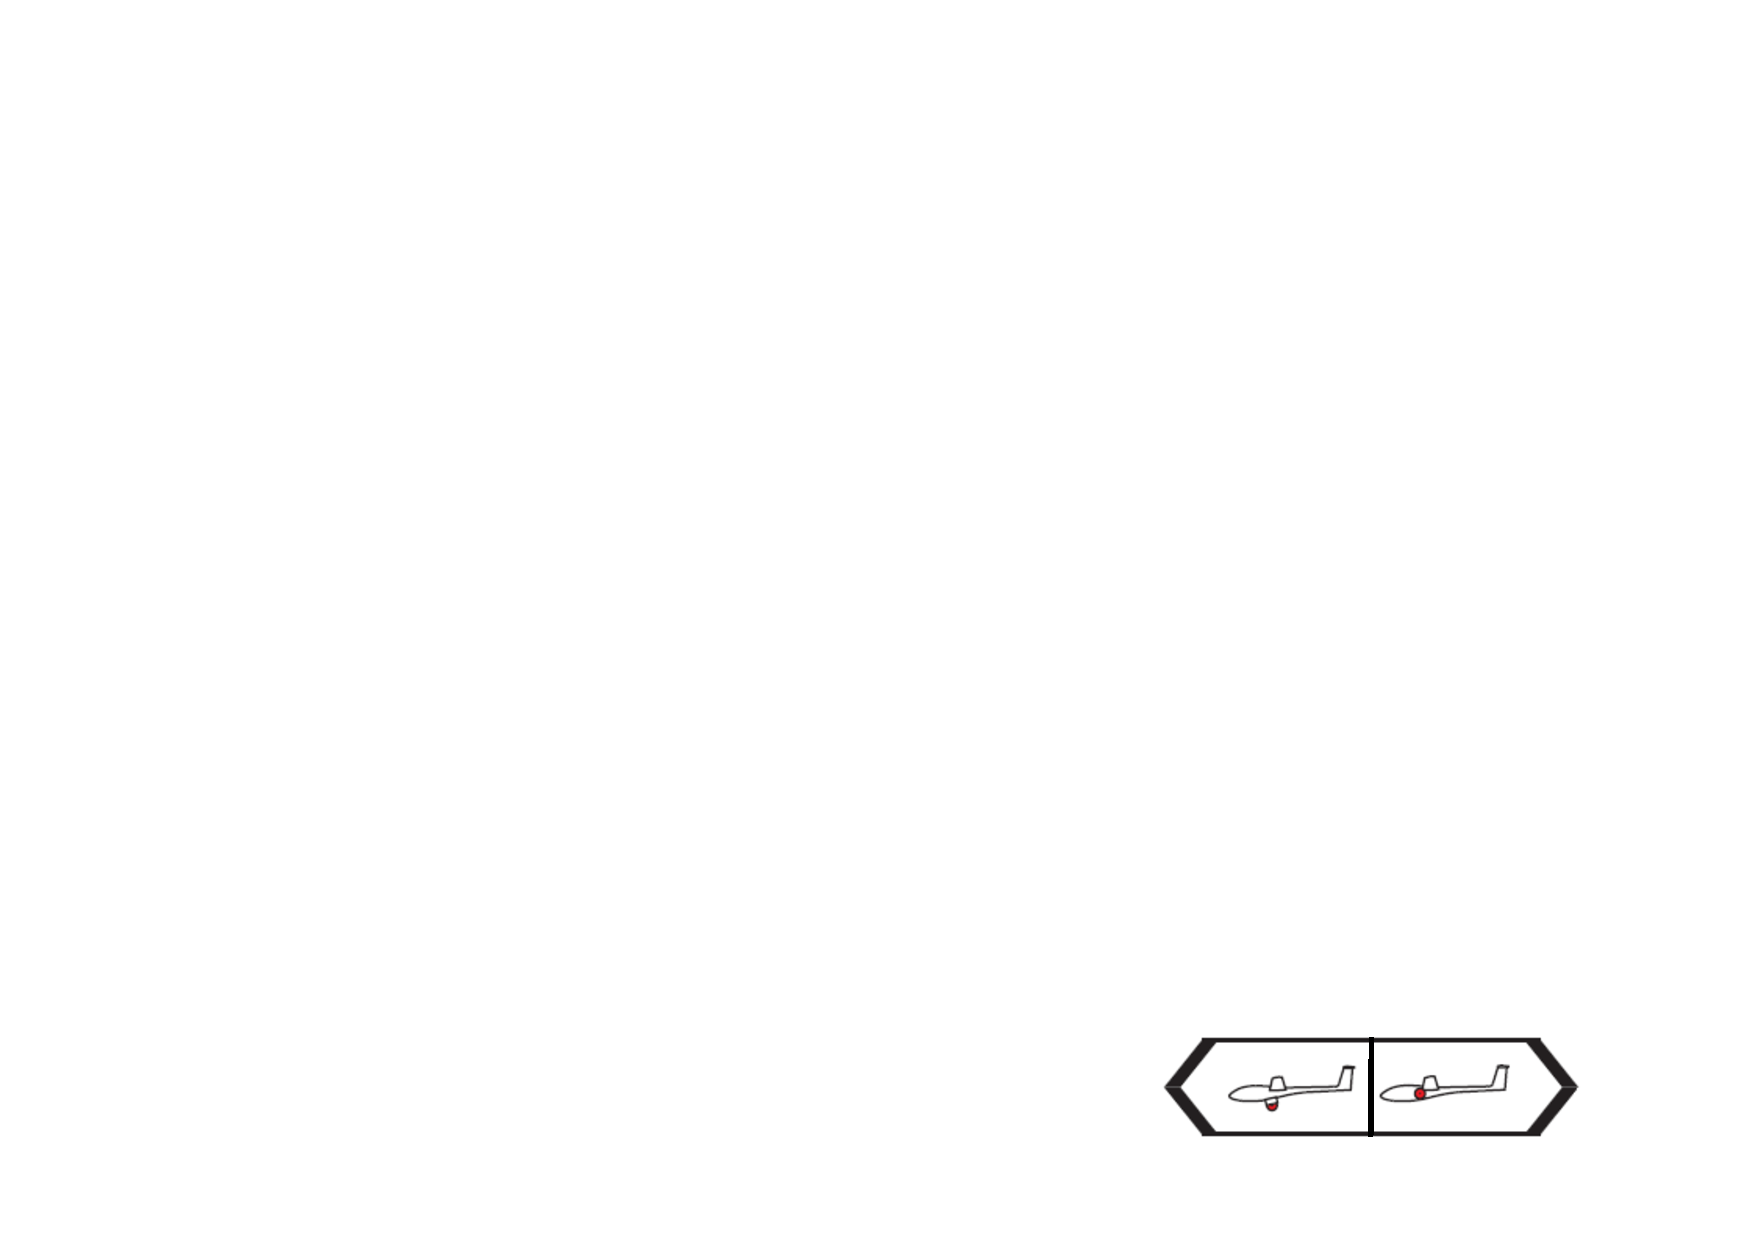
\includegraphics[width=.45\textwidth]{bilder/fahrwerk.pdf}
\caption*{Fahrwerk, silberner Hebel in der Mitte}
\end{center}
\end{figure}

\begin{figure}[H]
\begin{center}
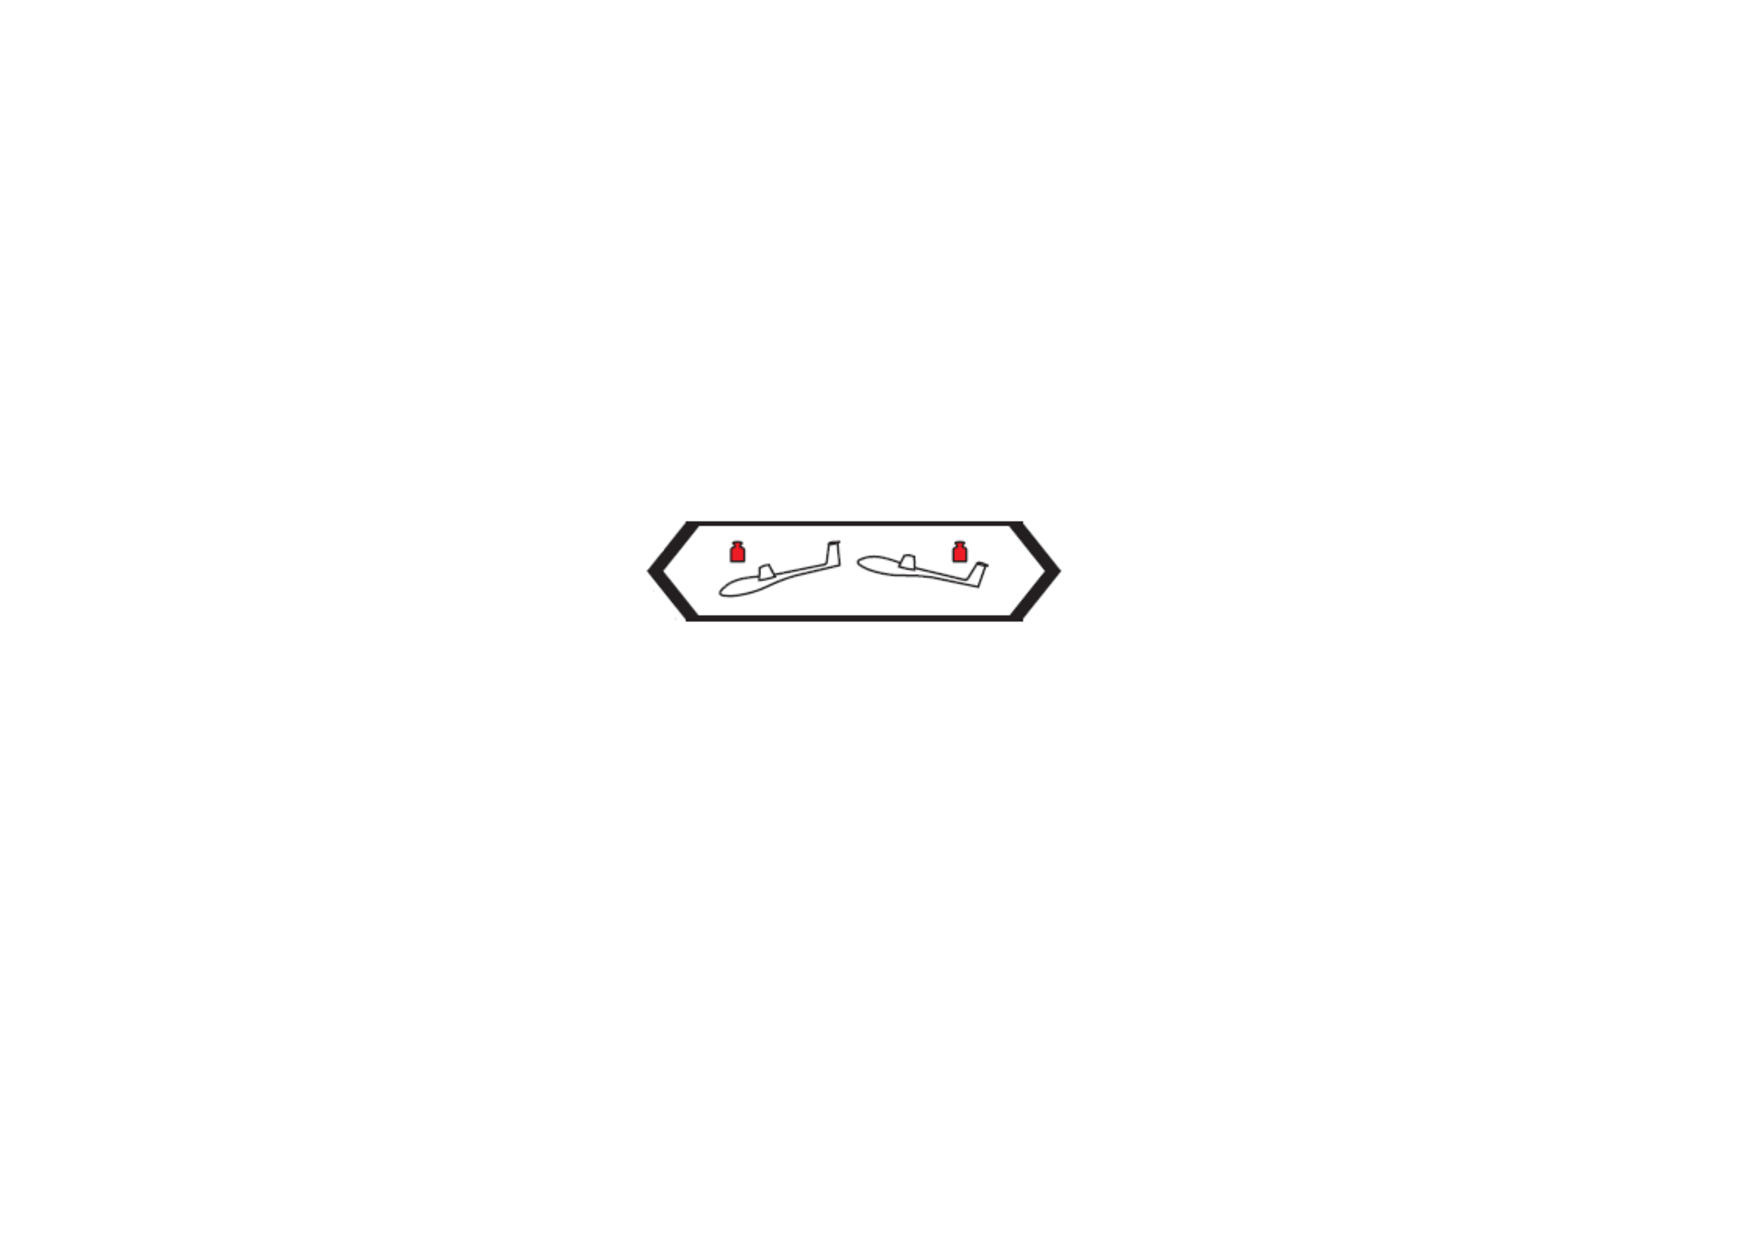
\includegraphics[width=.45\textwidth]{bilder/trimmung.pdf}
\caption*{Trimmung, grüner Hebel in der Mitte}
\end{center}
\end{figure}

\begin{figure}[H]
\begin{center}
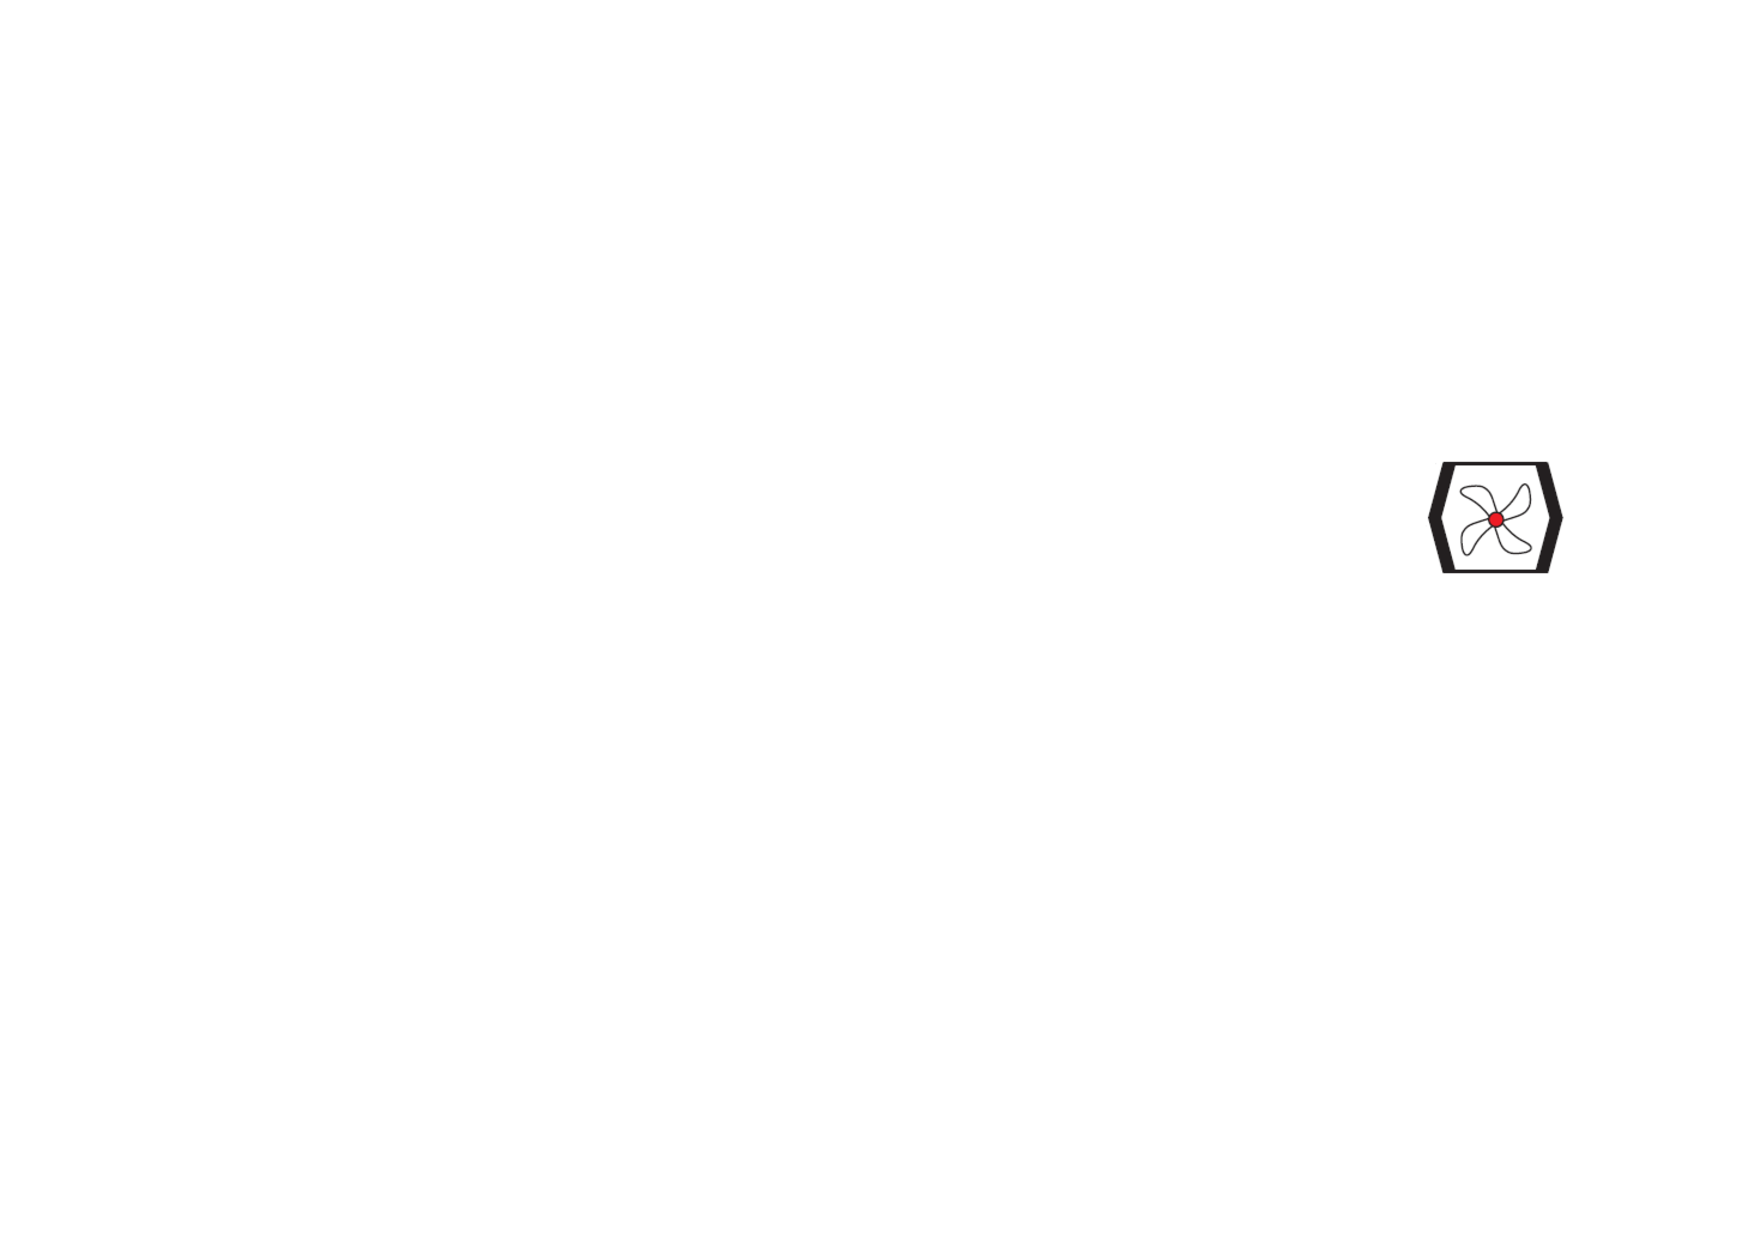
\includegraphics[width=.15\textwidth]{bilder/lueftung.pdf}
\caption*{Lüftungsbetätigung, Knopf links und rechts an Cockpitwand}
\end{center}
\end{figure}

\begin{figure}[H]
\begin{center}

\includegraphics[width=.15\textwidth]{bilder/kupplung.pdf}
\caption*{Schleppkupplung, gelber Griff jeweils links neben Steuerknüppel}
\end{center}
\end{figure}

\begin{figure}[H]
\begin{center}

\includegraphics[width=.15\textwidth]{bilder/pedale.pdf}
\caption*{Pedalverstellung, weißer Griff rechts neben Steuerknüppel}
\end{center}
\end{figure}

\begin{figure}[H]
\begin{center}

\includegraphics[width=.45\textwidth]{bilder/wk.pdf}
\caption*{Wölbklappenhebel, schwarzer Griff, jeweils links}
\end{center}
\end{figure}

Zusätzliche Hinweisschilder müssen für mit einem FES System ausgestattete
Segelflugzeuge hinzugefügt werden:\\

\begin{center}
\begin{tabular}[H]{|l|l|l|}
\hline
\multicolumn{2}{|l|}{\textbf{Geschwindigkeit IAS:}} & Km/h \\
\hline
Triebwerksbetrieb & $V_\text{PO}$ & 80-160 \\
\hline
Max. Motor Start/Stopp & $V_\text{POmax}$ & 135 \\
\hline
\end{tabular}
\end{center}



\chapter{ Notverfahren}
\pagecolor{red}
\section{Einführung}
Der vorliegende Abschnitt beinhaltet die Beschreibung der empfohlenen Verfahren bei eventuell eintretenden Notfällen.

\section{Abwerfen der Kabinenhaube}
Erfordert eine Situation das Abwerfen der Kabinenhaube, müssen folgende Schritte in der richtigen Reihenfolge ausgeführt werden:
\begin{itemize}
\item \textbf{Den roten Griff unten links auf dem Instrumentenbrett kräftig nach hinten bis zum Anschlag durchziehen}
\item \textbf{Haube nach oben wegstoßen}
\end{itemize}

Durch das Ziehen des roten Griffes am Instrumentenpilz wird die Haube an ihren seitlichen Befestigungen gelöst. Im vorderen Teil der Haubenmimik befinden sich zwei vorgespannte Federn, die nach dem Entriegeln die Haube vorne in die Strömung drücken. Die jetzt angreifenden Luftkräfte reißen die Haube nach hinten weg, wobei sie dabei eine definierte Drehung um die hintere Aufhängung (an der Gasdruckfeder) vollzieht. Diese Aufhängung ist mit einer Sollbruchstelle ausgestattet, die sich während oder unmittelbar nach der Drehung der Haube löst.\\
Falls nötig, muss die Haube zusätzlich mit beiden Händen nach oben weggedrückt werden.\\
\newline
\newline
\begin{color}{white}
\large{\underline{Wichtiger Hinweis}}\\
Bei ausgefahrenem Fahrwerk muss der Griff für den Haubennotabwurf leicht gedreht werden.
\end{color}\\

\begin{color}{white}
\large{\underline{Warnung}}\\
Vor dem Abwerfen der Kabinenhaube, wenn möglich den Motor
stoppen und das Antriebssystem ausschalten.
\end{color}

\section{Notausstieg}

Bei einem Notabsprung im Flug sollte man sich an die folgende Reihenfolge halten: 
\begin{enumerate}
\item \textbf{Haube} - abwerfen
\item \textbf{Gurtzeug} - öffnen
\item \textbf{Ausstieg} - mit beiden Armen über den Haubenrand hebeln (Körper möglichst anhocken) und dann vom Flugzeug abdrücken
\end{enumerate}

\begin{color}{white}
\large{\underline{Warnung}}\\
Vor dem Notausstieg, wenn möglich Motor stoppen und das Antriebssystem ausschalten.
\end{color}

\section{Beenden des überzogenen Flugzustands}
Der überzogene Flugzustand äußert sich bei einer Annäherung an die Mindestgeschwindigkeit (unabhängig von Wölbklappenstellung oder Querneigung) durch Weichwerden der Ruder, einer Taumelbewegung auf die eine Nickbewegung folgt, sowie Schütteln, Sackflug und Abreißerscheinungen am Rumpf.\\
\newline
\textbf{Dieser überzogene Flugzustand wird durch ein deutliches Nachlassen der Höhensteuerung und einer evtl. Verminderung der Querneigung beendet.}\\
\newline
Wird im Sackflug der Anstellwinkel durch weiteres "`Ziehen"' deutlich erhöht, kann je nach Schwerpunktlage "`Trudeln"' die Folge eines einseitigen Abkippens über den Flügel sein.\\

\textbf{Im Motorbetrieb muss zuerst der Motor gestoppt werden. Danach wird der überzogene Flugzustand gem. Flughandbuch beendet}
\newpage
\section{Beenden des Trudelns}
Im Rahmen der Flugerprobung wurde das Trudeln mit unterschiedlichen Schwerpunktlagen, Drehrichtungen und Wölbklappen"-stellungen eingeleitet.\\
Bei den Wölb"-klappen"-stellungen \textbf{$-2$}, \textbf{$-1$} und \textbf{$0$} beträgt die maximale Fahrt beim Ausleiten \textbf{$\unit[190]{\frac{km}{h}}$} und bei den Wölbklappenstel"-lung"-en \textbf{$+1$} und \textbf{$+2$} beträgt sie \textbf{$\unit[170]{\frac{km}{h}}$}.
\newline

\begin{color}{white} 
\underline{Warnung}\\
Bei der Wölbklappenstellung 'L' beträgt die zulässige Höchst"-ge"-schwin"-digkeit $\unit[130]{\frac{km}{h}}$. Da diese Geschwindigkeit beim Ausleiten schnell erreicht werden kann, sollte man vor dem Ausleitvorgang eine andere Wölbklappenstellung rasten, um die Flugzeugstruktur nicht zu überlasten.\\
\end{color}


Um das Trudeln auszuleiten, kann bei der B13 die Standardmethode angewandt werden. Im Falle des Motorbetriebes, muss dieser zunächst gestoppt werden.

\begin{enumerate}
\item \textbf{Motor ggf. stoppen}
\item \textbf{Seitenruder gegen die Trudelrichtung}
\item \textbf{Höhenruder neutral stellen}
\item \textbf{Warten bis die Drehung aufhört}
\item \textbf{Seitenruder neutral stellen}
\item \textbf{Vorsichtig abfangen}
\end{enumerate}


\begin{color}{white}
\underline{Wichtiger Hinweis}\\
Der Höhenverlust kann beim Ausleiten bis zu $\unit[200]{m}$ betragen!
\end{color}

\section{Beenden des Spiralsturzes}
Beim Trudeln wurde in keinen der durchgeführten Erprobungsszenarien eine Neigung zum Spiralsturz erkennbar.\\
Sollte sich trotzdem ein Spiralsturz einstellen, kann man ihn mit folgenden Steuereingaben ausleiten:
\begin{enumerate}
\item \textbf{Motor stoppen}
\item \textbf{Quer- und Seitenruder in Gegendrehrichtung}
\item \textbf{Vorsichtig Fahrt abbauen}
\end{enumerate}

\begin{color}{white}
\underline{Warnung}\\
Beim Abfangen sind die zulässigen Ruder- und Klappenausschläge zu den erreichten Geschwindigkeiten zu beachten.
\end{color}

\section{Notlandungen}
\subsection{Notlandung mit eingezogenem Fahrwerk}
Notlandung immer mit ausgefahrenem Fahrwerk, da der Pilot und die Flugzeugstruktur durch die Arbeitsaufnahme des gefederten Fahrwerks erheblich besser geschützt sind, als nur durch die Rumpfschale.\\
\newline
Lässt sich das Fahrwerk nicht ordnungsgemäß ausfahren, dann ist das Flugzeug in \textbf{Landestellung L der Wölbklappen} und mit \textbf{eingefahrenen Bremsklappen} in einem \textbf{flachen Winkel mit Mindestfahrt} aufzusetzen, um ein Durchsacken zu vermeiden.\\
Nach der Landung sollte eine gründliche Kontrolle der Flugzeugstruktur erfolgen.

\subsection{Notlandung auf dem Wasser}
Aus den bei Notlandungen auf Wasser gemachten Erfahrungen muss mit der Möglichkeit gerechnet werden, dass das gesamte Cockpit unter Wasser gedrückt wird. Bei Wassertiefen $>\unit[2]{m}$ sind die Insassen in höchster Gefahr! Deshalb sollte die Notwasserung nur als letzter Ausweg gewählt werden.\\
\newline
Folgendes Vorgehen wird bei einer Notwasserung empfohlen:
\begin{itemize}
\item \textbf{Fahrwerk ausfahren}
\item \textbf{Fallschirmgurte öffnen}
\item \textbf{Aufsetzen mit ausgefahrenem Fahrwerk und möglichst geringer Geschwindigkeit}
\item \textbf{Das Cockpit sollte durch die Notfenster geflutet werden, um gegen den Wasserdruck die große Haube öffnen zu können}
\item \textbf{Nach dem Eintauchen Gurtzeug und Fallschirm ablegen}
\end{itemize}

\subsection{Drehlandung ("`Ringelpietz"')}
Wenn abzusehen ist, dass ein Landefeld von der Länge her nicht ausreicht, dann ist spätestens $\unit[50]{m}$ vor Ende des Landefeldes eine gesteuerte Drehlandung einzuleiten:
\begin{enumerate}
\item \textbf{Flügel zur Ausweichrichtung hin auf den Boden steuern}
\item \textbf{Wenn möglich in den Gegenwind drehen}
\item \textbf{Gleichzeitig durch Nachdrücken den Sporn entlasten und durch gegensinniges Seitenruder der Torsion der Rumpfröhre entgegenwirken.}
\end{enumerate}


\section{Flug im Bereich von Gewittern}
Durch Blitzschlag sind wiederholt Kohlenstofffaserstrukturen zerstört worden. Flüge und besonders Windenschlepps im Bereich von Gewittern sind daher unbedingt zu vermeiden, da in wichtigen Strukturen der B13 Kohlenstofffasern verwendet werden.\\
Wenn der Verdacht auf Blitzschlag besteht oder ein solcher erfolgt ist, sollte die Fahrt auf \textbf{unter $V_A=\unit[160]{\frac{km}{h}}$} reduziert werden. Die \textbf{Ruderwirksamkeit} ist zu \textbf{überprüfen} (Gefahr des Verschweißens der Rudergelenke) und \textbf{elektrische Systeme} sind \textbf{auszuschalten} um Kabelbrand zu vermeiden.
Zusätzlich sind der \textbf{Propeller einzufahren} und die \textbf{Nasenklappen zu schließen}, um das Eindringen von Wasser in den Motorraum zu verhindern.



\section{Flug bei Regen}
Flüge in starkem Regen und Gewittern sind zu vermeiden. Es wird empfohlen den Propeller einzufahren und die Nasenklappen zu schließen, um das Eindringen von Wasser in den Motorraum zu verhindern.
Wenn nötig ist ein Flug in leichtem Regen mit laufendem Motor möglich. Es sollte allerdings mit niedriger Leitungseinstellung geflogen werden, die ausreichend für den Horizontalflug ist, um Beschädigungen der Propellerblätter zu vermeiden. Bei starkem Regen muss der Motorbetrieb eingestellt werden. \\

Bei Regen verschlechtern sich die Flugleistungen. Es muss mit verstärktem Eigensinken und einer erhöhten Mindestfahrt gerechnet werden. Die Geschwindigkeit im Landeanflug sollte daher mindestens um $\unit[10]{\frac{km}{h}}$ erhöht werden. 

\section{Flug bei Vereisungsbedingungen}
Bei Vereisungsgefahr Gängigkeit der Ruder und Klappen durch ständiges Bewegen aufrechterhalten.
\newpage
\section{Triebwerksausfall}
\subsection{Motor startet nicht}
Falls der Motor nicht startet, muss der Flug im reinen Segelflug fortgesetzt werden. \\

\begin{color}{white}
\large{\underline{Anmerkung}}\\
Überprüfen, ob der Leistungsschalter eingeschaltet ist. Die Erinnerung (auf der FCU) “Check Power Switch” sollte ab einer bestimmten Leistungseinstellung erscheinen.
\end{color}

\subsection{Leistungsverlust während des Fluges}

Bei einem Leistungsverlust während des Fluges Steuerknüppel vorsichtig nach vorne drücken, um die gewünschte Fluggeschwindigkeit beizubehalten! Anschließend wie folgt verfahren:

\begin{enumerate}
\item Überprüfen, ob der Leistungsschalter unbeabsichtigt ausgeschaltet wurde! \\

In diesem Fall den Leistungsschalter wieder einschalten und die Leistung mit dem
Leistungsdrehregler anpassen.\\
\item Trifft Punkt 1 nicht zu, folgendermaßen fortfahren:\\
\begin{enumerate}
\item Zuerst den Leistungsschalter, dann die FCU ausschalten. \\
\item Schalten Sie die FCU wieder ein und überprüfen Sie, ob sich etwas ungewöhnlich verhält.\\

Wenn alles in Ordnung ist, Leistungsschalter wieder einschalten und Motor starten.
Wenn der Motor startet und sich unter Last ungewöhnlich verhält:
\begin{enumerate}
\item Drehenden Propeller mit der elektrischen Bremse anhalten.
\item Nachdem der Propeller gestoppt ist, zuerst den Leistungsschalter und dann die FCU ausschalten.
\end{enumerate}

Sollte der Propeller nicht gestoppt werden können, kann der Propeller mit dem Noteinfahrmechanismus abgebremst und eingefahren werden.
\end{enumerate}
\end{enumerate}

Noteinfahrmechanismus:
\begin{enumerate}
\item Engine Swich ausschalten
\item Sicherheitspin aus Schlittenhauptschalter herausziehen
\item Fluggeschwindigkeit verringern auf $\unit[80]{km/h}$ soweit möglich
\item Schlittenhauptschalter wiederholt kurzzeitig nach hinten drücken. Dies aktiviert den Schlittenmotor und zieht den Propeller gegen den Bremsgummiring
\item Sobald der Propeller abgebremst und eingeklappt ist, kann das Schlittensystem wieder normal in Betrieb genommen werden und der Propeller normal eingefahren werden.
\end{enumerate}

\begin{color}{white}
\large{\underline{Warnung}}\\
Der Propeller kann beim Noteinfahren beschädigt werden! Wiederinbetriebnahme des Antriebssystems erst nach gründlicher Inspektion aller Bauteile.
\end{color}\\

Sollte dieser Noteinfahrmechanismus nicht funktionieren, muss mit drehendem Propeller gelandet werden. In diesem Fall muss bei der Landung vorsichtig und gleichzeitig auf beiden Rädern aufgesetzt werden (Zweipunktlandung), um eine Beschädigung des Propellers zu verhindern.\\

\begin{color}{white}
\large{\underline{Anmerkung}}\\
Eine Graspiste in gutem Zustand (ohne Schlaglocher oder Ähnlichem) ist einer Asphaltpiste vorzuziehen.
\end{color}\\

\begin{color}{white}
\large{\underline{Warnung}}\\
Landungen in hohem Bewuchs sind zu vermeiden.
\end{color}\\

\begin{color}{white}
\large{\underline{Anmerkung}}\\
Der Verlust der Gleitleistung durch den drehenden Propeller ist gering. Daher besteht bei ausreichend Höhe genug Zeit ein geeignetes Landefeld zu wählen.
\end{color}\\

Bitte lesen Sie das \textbf{FES FCU INSTRUMENTENHANDBUCH} für das Verhalten und die notwendigen Verfahren beim Erscheinen von bestimmten Nachrichten und Aufblinken von LED-Leuchten.

\section{Brand}
\subsection{Brand am Boden}

\begin{itemize}
\item Leistungsschalter ausschalten und alle Instrumente, sowie den Hauptschalter ausschalten
\item Cockpit verlassen
\item Brand löschen
\end{itemize}
\newpage
\subsection{Brand während des Fluges}
\begin{itemize}
\item Motor sofort abstellen
\item Leistungsschalter ausschalten und vordere Lüftung, falls noch nicht geöffnet, öffnen
\item Seitliches Haubenfenster offnen
\item So schnell wie möglich landen (oder gegebenenfalls einen Notausstieg in Betracht ziehen)
\item Nach der Landung Feuer löschen
\end{itemize}

\section{Sonstige Notfälle}

\subsection{Verlust der 12V Spannungsversorgung während des Fluges}

Segelflug:\\
Beim Ausfall der elektrischen Instrumente (Funkgerät, Bordrechner, FCU etc.)
wahrend des Segelfluges, muss der Flug im reinen Segelflug fortgesetzt werden. In
diesem Fall kann der Propeller nicht ausgefahren werden und der Motor nicht gestartet werden.\\

Ist die FCU nicht vom Ausfall betroffen, kann der Motorstart bei Bedarf versucht werden.\\

Motorflug:\\
Beim Ausfall der FCU während des Motorfluges, fällt auch der Motor aus. Ein Stoppen des drehenden Propellers durch die Noteinfahrfunktion möglich.\\

Fallen die Instrumente nur teilweise aus und ist die Funktion von FCU und Motor nicht beeinträchtigt, kann der Motor weiter betrieben werden.

\chapter{ Normale Betriebsverfahren}
\pagecolor{white}
\section{Einführung}
Dieser Abschnitt enthält Checklisten und Beschreibungen für die tägliche Kontrolle und Vorflugkontrolle, sowie für die normalen Betriebsverfahren. Normale Verfahren im Zusammenhang mit Zusatzausrüstung sind im Abschnitt 9 beschrieben.


\section{Montageverfahren, Laden, Ein- und Ausbau der Akkupacks}
Die B13 lässt sich mit Hilfe einer Flächenstütze durch vier Personen auf- und abrüsten. Die Batterien können nur im abgerüsteten Zustand ein- und ausgebaut werden.

\subsection{Auf- und abrüsten}
Das Aufrüsten der B13 geschieht in folgender Reihenfolge.\\
\newline
\underline{Vorbereitungen}
\begin{itemize}
\item Transportanhänger sichern
\item alle Bolzen und Buchsen säubern und fetten
\item Trimmung kopflastig stellen, Wölbklappen auf Stellung 0 bringen und Bremsklappen entriegeln
\item Batterie in Halterung einbauen und anschließend
\item Gepäckfach einbauen

\end{itemize}

\underline{Innenflächen}
\begin{itemize}
\item Linken Hauptbolzen in das Auge des linken Innenflügels stecken
\item Linken Holmstummel bis zur Hälfte einführen
\item Rechten Hauptbolzen in das vorgesehene Auge stecken
\item Linke Innenfläche in den Rumpf stecken und beide Hauptbolzen bis zum Querkraftrohr herausziehen
\item Rechten Innenflügel in den Rumpf stecken
\item Hauptbolzenachsen zum Fluchten bringen (dies ist nur möglich, wenn beide Flügel bis an den Rumpf eingeführt sind), Hauptbolzen eindrücken und sichern. Graue Markierung auf rechten Holmstummel kann bei der Ausrichtung der Flügel helfen. (untere Kante parallel zu Holmstummeloberkante)
\item Steuerung im Rumpf anschließen und sichern - \begin{color}{red} 2x3 Anschlüsse. (L'Hotellier) \end{color} Es kann hilfreich sein, die Querruderanschlüsse im Rumpf erst nach Montage der Außenflächen anzuschließen.
\item Sicherungsschraube am Rechten Hauptbolzen lässt sich am besten einführen, wenn Hauptbolzengriff nach unten steht, danach Hauptbolzen in vorgesehene Sicherung einrasten und Sicherungsschraube mit Fokkernadel sichern.
\end{itemize}

\underline{Außenflächen}
\begin{itemize}
\item Außenflächenbolzen-Tool in das vorgesehene Loch des Außenflächenbolzens einführen
\item Außenfläche bis auf $\unit[10]{cm}$ in die Innenfläche einführen
\item Querruder anschließen und sichern \begin{color}{red} (L'Hotellier) \end{color}
\item Außenfläche vollständig einführen
\item Außenflächenbolzen von vorne in die Bohrung einführen
\item Außenflächenbolzen-Tool entfernen und mit dem federbelasteten Sicherungsstift die Außenflächen-Bolzen sichern 
\end{itemize}

\underline{Höhenleitwerk}
\begin{itemize}
\item M3-Montageschraube mit roter Kugel in den vorderen Anschlussbolzen an der oberen Seitenflossen-Vorderkante einschrauben
\item Höhenleitwerk auf beide Antriebsbolzen aufstecken und ganz nach hinten schieben
\item Montageschraube ziehen, das Leitwerk senkt sich ab und wird vom vorderen Anschlussbolzen gesichert, in dem die Montageschraube wieder losgelassen wird
\item Montageschraube herausschrauben (nach Herausschrauben, darf der Bolzen nicht mehr aus der Vorderkanten-Kontur der Seitenflosse herausstehen), Gewindeöffnung abkleben
\end{itemize}

\underline{Nachbereitungen}
\begin{itemize}
\item Düse in die Düsenaufname der Seitenflosse schieben
\item Antennenkabel an der Haube anschließen
\item Querruder, Wölbklappen, Bremsklappen, Höhenruder, Seitenruder auf Sicherung, Funktion und Freigängigkeit überprüfen
%\item Batterie in der vorgesehenen Halterung (hinter dem rechten Piloten) befestigen
\item Alle Trennstellen (Innenfläche-Außenfläche, Rumpf-Innenfläche, Seitenleitwerk-Höhenleitwerk) mit Isolierband abkleben
\end{itemize}
\begin{color}{red}
\large{\underline{Warnung}}\\
Bei den Ruderanschlüssen handelt es sich um manuelle Anschlüsse (L'Hotellier). Sie sind zu sichern (Federstecker) und vor jedem Flugbetrieb auf richtigen Anschluss und Sicherung zu kontrollieren!
\end{color}\\

Das Abrüsten geht in umgekehrter Reihenfolge wie das Aufrüsten vonstatten.

\subsection{Laden der Akkupads}

Die Betriebsanweisung zum Laden der Akkupacks ist im separaten \textbf{FES
AKKUPACKHANDBUCH} beschrieben.\\

Das Aufladen der Akkupacks kann auch optional ohne Ausbauen der Akkus erfolgen. Hierfür wurden separate Ladestecker mittig hinter den Pilotensitzen montiert. 
Die Ladegeräte werden hierfür mit speziellen Adapterkabeln mit den Ladebuchsen der B13 verbunden, die Datenkabel der Ladegeräte werden mit der vorgesehenen „CHARGE“ Buchse auf der Batteriefirewallabdeckung verbunden.\\

\begin{color}{blue}
\large{\underline{Anmerkung}}\\
Es wird empfohlen die Akkupacks erst ein bis zwei Tage vor
dem geplanten Flug vollständig zu laden. Es soll jedoch immer genug Zeit
eingeplant werden, um einen vollständigen Ladeprozess zu garantieren!
\end{color}

\subsection{Einbau der Akkupacks in das Segelflugzeug}

\begin{color}{red}
\large{\underline{Warnung}}\\
Vor dem Einbau muss sichergestellt werden, dass beide
Akkupacks vollständig geladen sind. Beide Akkupacks müssen annähernd die
gleiche Spannung pro Zelle haben (ca. $\unit[4,16]{V}$ pro Zelle). Die Abweichung der
Gesamtspannung beider Akkupacks darf maximal $\unit[0,4]{V}$ betragen.\\
FES FLUGHANDBUCH Version 1.15 November 2016\\
Seite 17 von 34
\end{color}

Zum Einbau der Akkus wird wie folgt vorgegangen:

\begin{enumerate}
\item Akkufachabdeckung öffnen.
\item Kontrollieren, dass der Leistungsschalter ausgeschaltet ist.
\item Prüfen, dass die FCU und alle anderen Instrumente (Flugrechner, Flarm, Funk,
Transponder, PDA etc.) ausgeschaltet sind.
\item Das erste Akkupack mit dem Bedienterminal nach vorne in den Rumpf einführen und nach hinten schieben.
\item Das zweite Akkupack mit Bedienterminal nach hinten in den Rumpf einführen.
\item Ein Halteplattenpaar auf dem hinteren Akkupack mittig über dem Haltegurt positionieren und die Schraube von Hand anziehen.
\item Ein Halteplattenpaar auf dem vorderen Akkupack mittig über dem Haltegurt positionieren und die Schraube von Hand anziehen.
\item Stromkabel aus der Seitenhalterung nehmen.
\item Das kürzere Kabel mit dem $\unit[8]{mm}$ Stecker und dem SCHWARZEN Gehäuse in die mit minus markierte Buchse des vorderen Akkupacks einstecken.
\item Das längere Kabel mit dem $\unit[10]{mm}$ Stecker und dem ROTEN Gehäuse in die mit plus markierte Buchse des hinteren Akkupacks einstecken.
\item Die Stecker des Datenkabels in jeden Akkupack in den passenden DATA Anschluss einstecken.
Vor dem Einstecken vergewissern, dass die Orientierung richtig herum ist.
Die Stecker müssen gerade eingesteckt werden, ansonsten können die Pins verbogen werden.
\item “BMS Schalter” an jedem Akkupack einschalten und warten bis der Testlauf abgeschlossen ist.
\item Akkufachabdeckung schließen.
\end{enumerate}

\section{Tägliche Kontrolle}
Vor Beginn des Flugbetriebes muss die B13 anhand der folgenden Checkliste sorgfältig überprüft werden. Insbesondere für die Ruderproben empfiehlt sich die Unterstützung durch eine zweite Person.\\
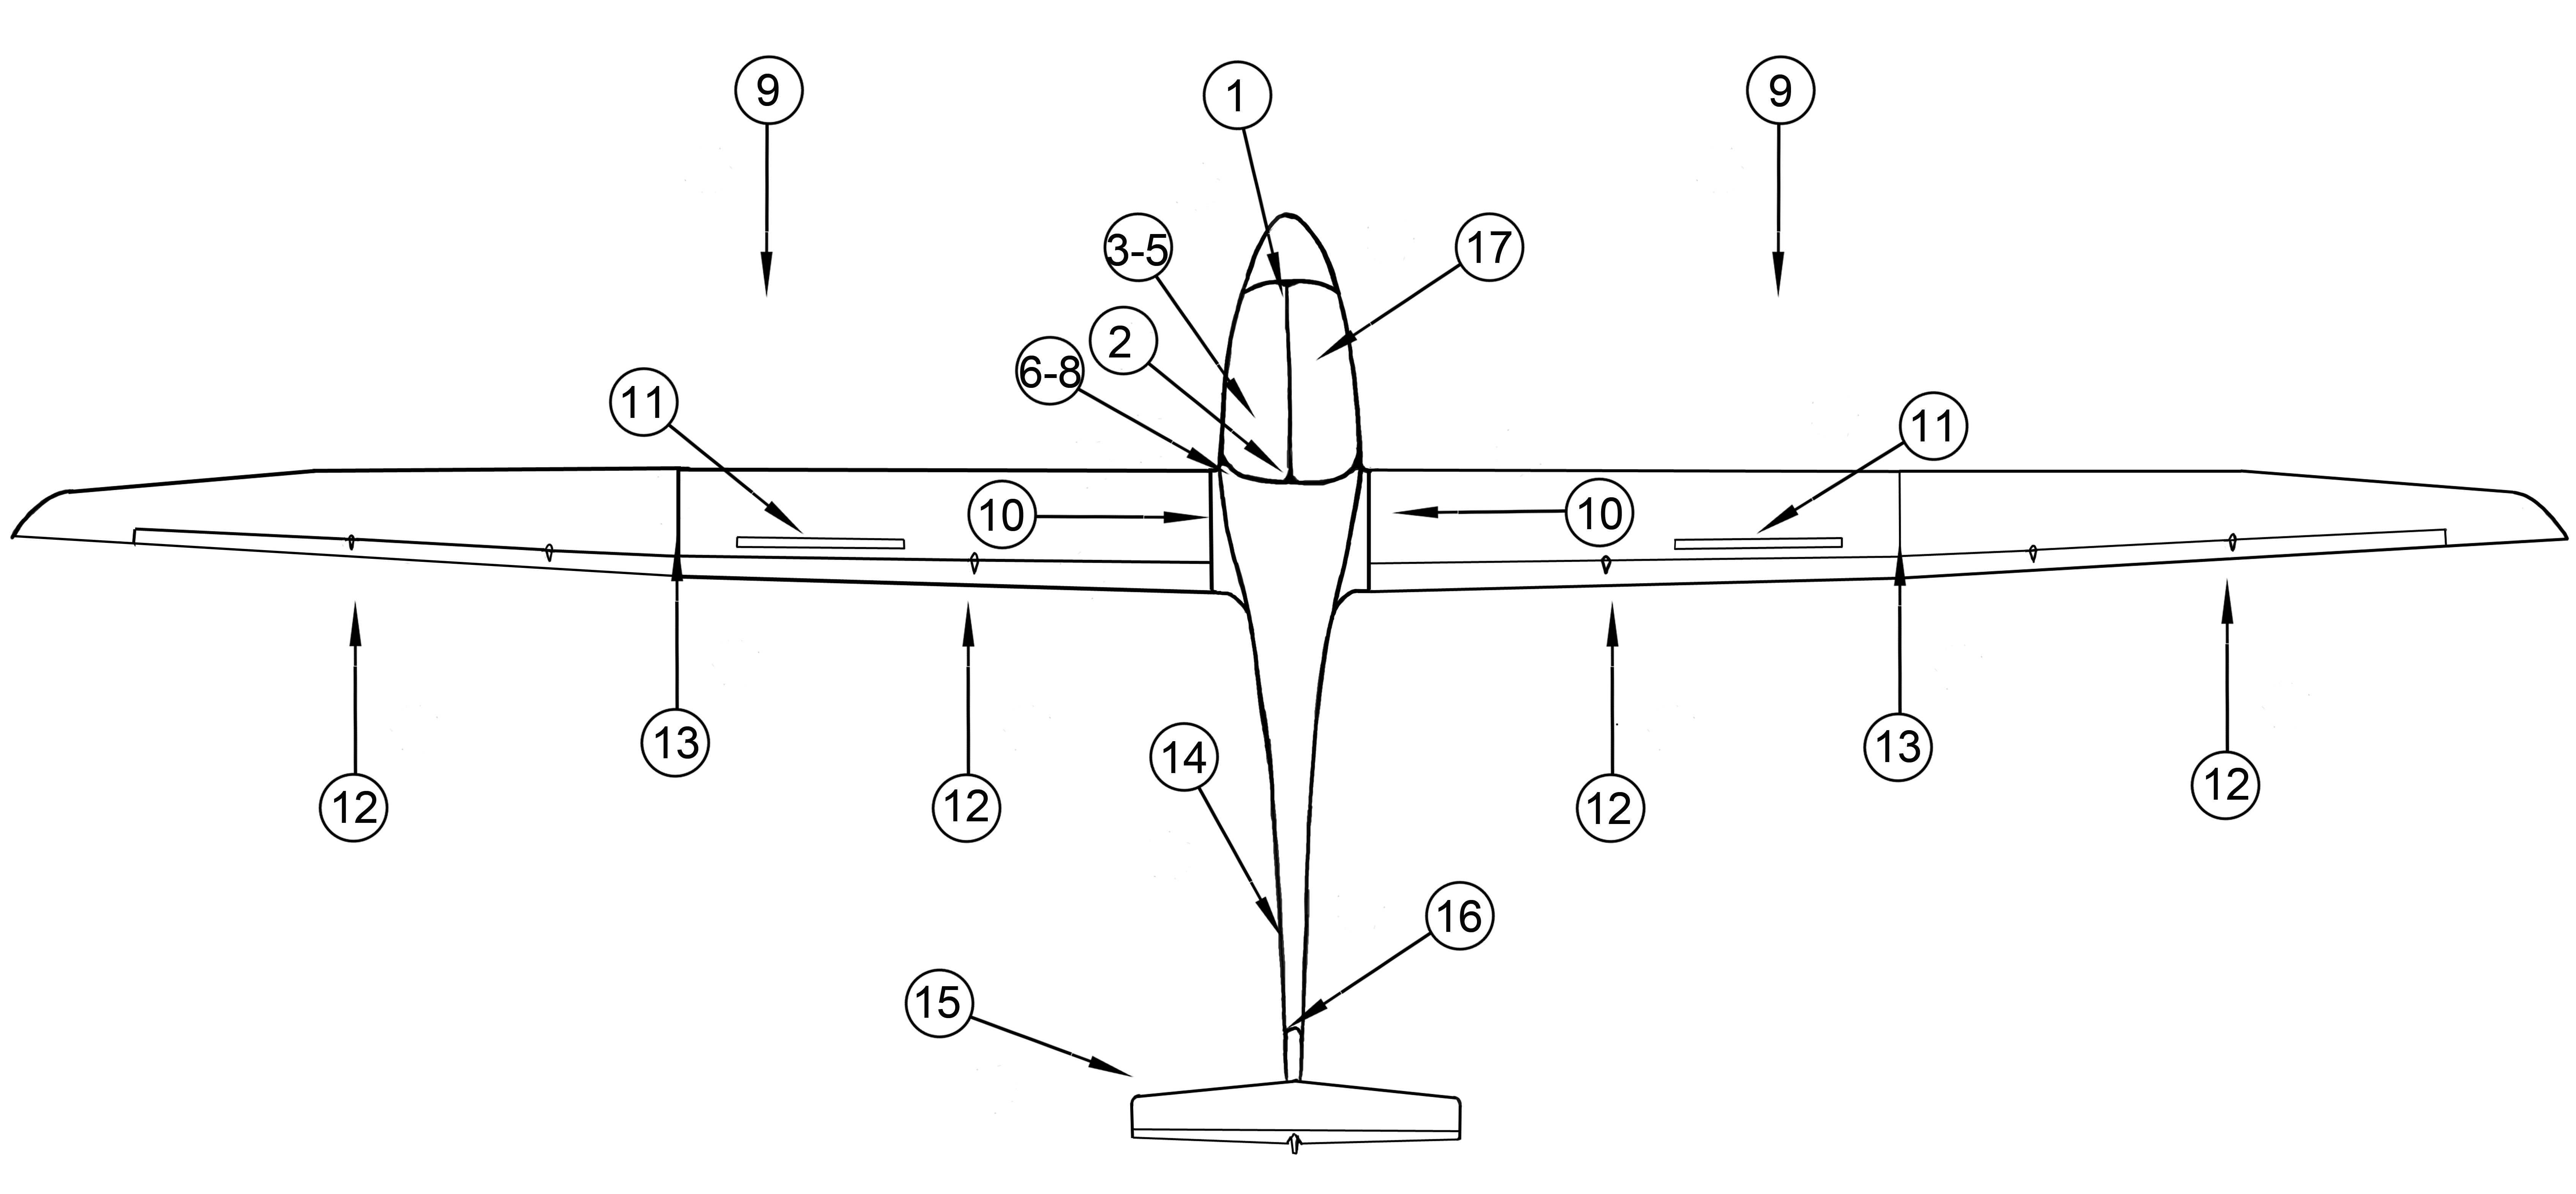
\includegraphics[width=\textwidth]{b13check.png}
\begin{enumerate}
\item Haube öffnen und Haubennotabwurf überprüfen
\item Sicherung der Hauptbolzen überprüfen
\item Fremdkörperkontrolle im gesamten Cockpitbereich
\item Freigängigkeit und Spielfreiheit aller Bedienelemente prüfen
\item Ruderprobe bei allen Rudern (Quer-, Seiten- und Höhenruder) und Klappen (Wölb- und Bremsklappe) unter Belastung durchführen. Sicherungen der Steuerung soweit einsehbar und erreichbar, überprüfen
\item Ausklinkprobe der Schleppkupplung, auch unter Last
\item Fahrwerk und Reifen auf Beschädigungen überprüfen, Luftdruck im Reifen prüfen (auch Spornrad), Rutschmarke
\item Radbremse auf Funktion und Dichtigkeit überprüfen, Abnutzungsgrad der Bremsbeläge prüfen
\item Flügelober- und Unterseite auf Beschädigungen (Lackrisse, o.ä.) überprüfen, besonders im Bereich der Flügelwurzel
\item Flügelanschlüsse auf besonderes Spiel in den Querkraftlagern prüfen
\item Bremsklappen auf Funktion, vollständiges Schließen der Abdeckungen, Fremdkörper oder Feuchtigkeit in den Kästen überprüfen
\item Flügelklappen und Anlenkungen überprüfen (Freigängigkeit, Spielfreiheit)
\item Außenflügelanschluss - Verriegelung und Sicherung überprüfen
\item Rumpfunterseite und Leitwerksträger auf Schäden (Lackrisse, etc.) 	überprüfen, besonders im Bereich der Leitwerksanschäftung (Kuller entfernen)
\item Seiten- und Höhenleitwerk auf richtige Montage, Spiel und Beschädigungen 	überprüfen, Seilzüge des Seitenruders prüfen
\item Druckabnahmen in der Seitenflosse (Dreifachdüse) überprüfen (mit 	Fahrtmesser und Variometer)
\item Elektrisches System (Funk, Rechner) überprüfen, 	Funkprobe
\end{enumerate}

Zusätzlich ist zu Beginn jedes Flugtages und nach jedem Einbau der Akkupacks die tägliche
Kontrolle durchzufuhren. Dazu gehören mindestens die nachfolgend aufgeführten Punkte.
Werden Probleme festgestellt, so darf auf keinen Fall gestartet werden, bevor diese
Probleme nicht fachgerecht beurteilt bzw. repariert wurden.

% noch nicht vollständig
\begin{itemize}
\item Das Antriebssystem muss einer optischen Kontrolle unterzogen werden. Insbesondere der Zustand der Propellerblätter, Schlittenmechanik sowie aller Hochstromverschlüsse muss überprüft werden
\item  Füllstand des Kühlsystems muss zwischen Min und Max sein
\end{itemize}

\section{Vorflugkontrolle}
Die folgende Checkliste ist im Cockpit für beide Piloten gut sichtbar angebracht. Anhand ihrer ist vor jedem Start eine Vorflugkontrolle durchzuführen:
\begin{center}
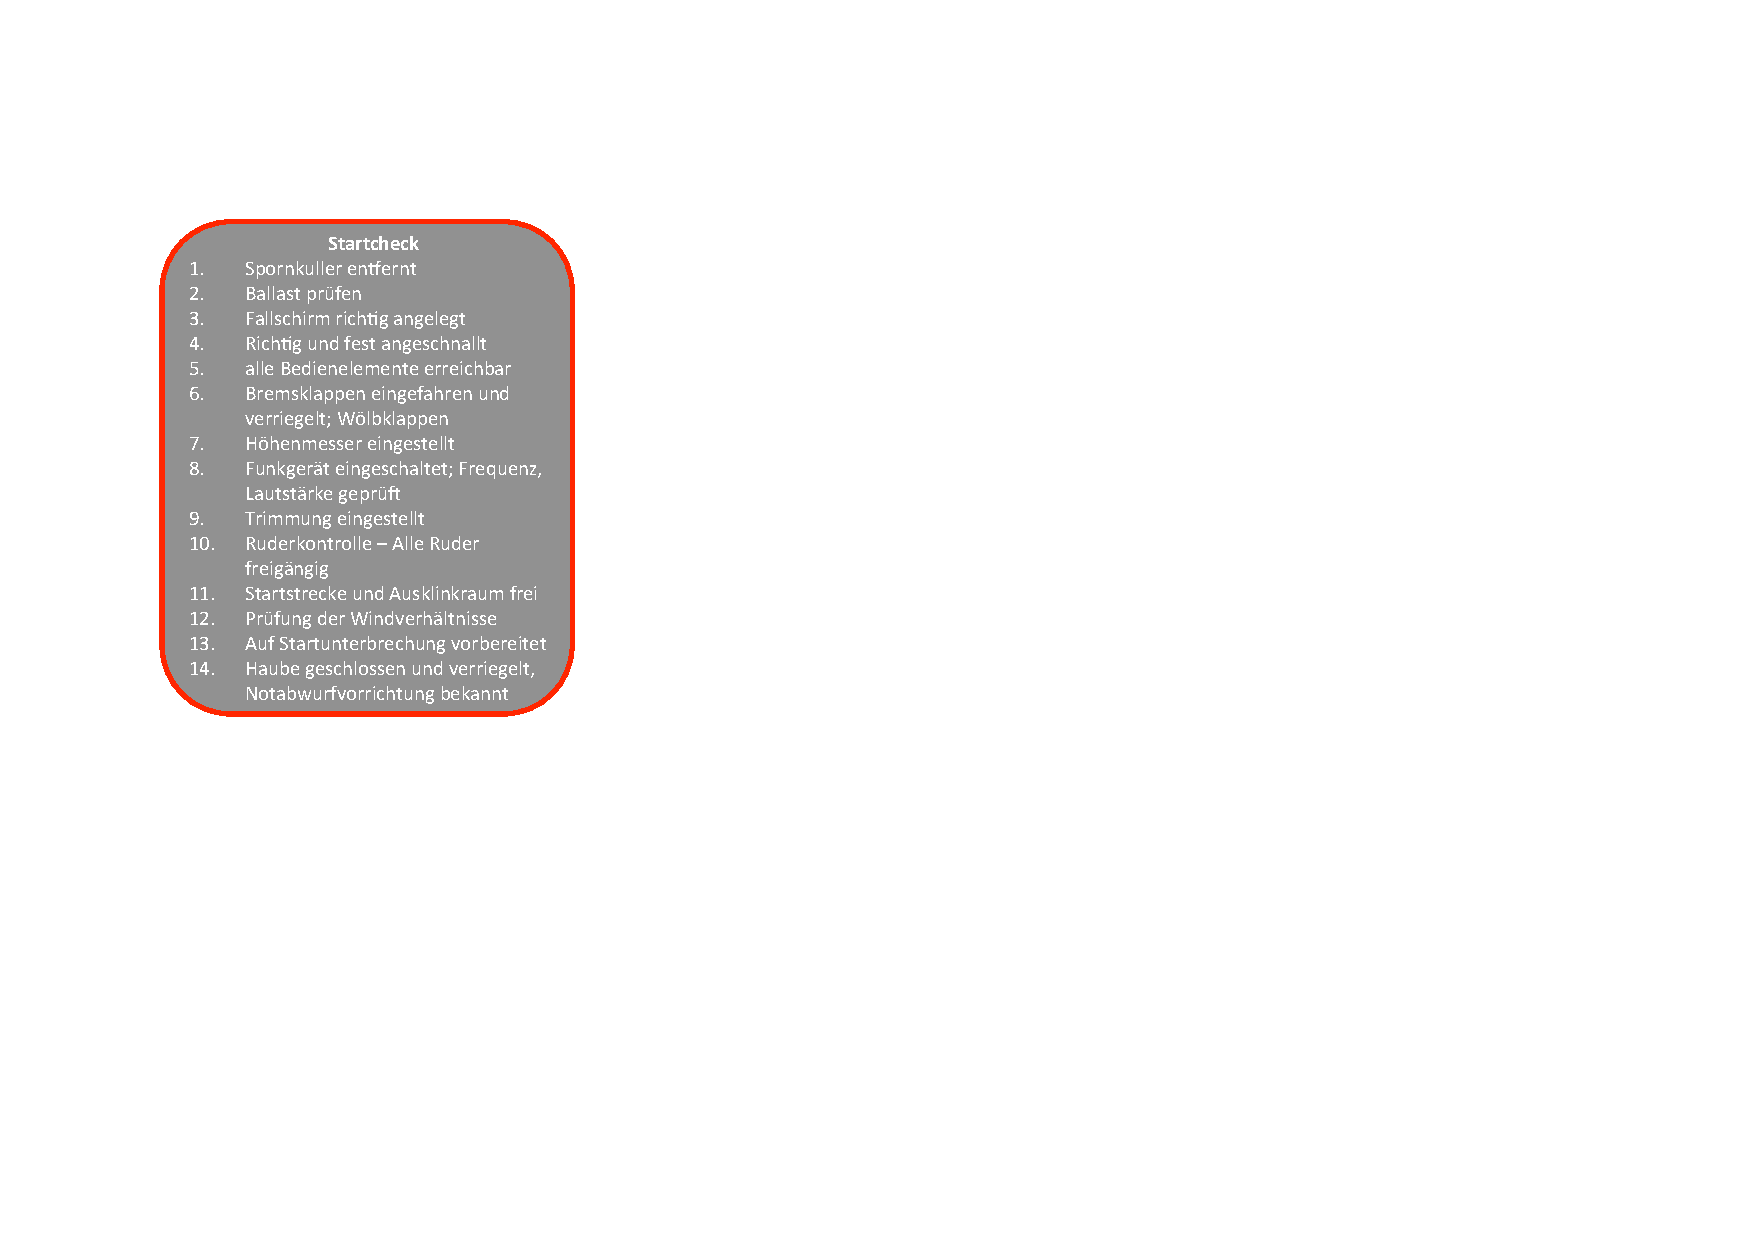
\includegraphics[width=.45\textwidth]{bilder/startcheck.pdf}
\end{center}

\subsection{Starten des Motors am Boden}

\begin{enumerate}
\item Sicherstellen, dass der \glqq ENGINE\grqq\ Schalter ausgeschaltet ist.
\item Heckkuller entfernen
\item Hochstrom Batterieanschlüsse an den Firewallboxen überprüfen. (Fester Sitz, Kabel bis zur Markierung eingesteckt)
\item CAN Bus Kabel an der Batteriefirewall auf festen Sitz überprüfen.
\item Propellerschlittensystem einschalten und warten bis alle Statuslampen Blau leuchten
\item Propeller durch Drücken des \glqq Extract\grqq-Schalters ausfahren. Warten bis alle Statuslampen grün anzeigen.
\end{enumerate}

\textbf{Tägliche Kontrolle vor dem Start: \\}
\begin{itemize}
\item Batterien geladen, korrekt eingebaut und angeschlossen?
\item Avionik Hauptschalter einschalten
\item Propellerschlittensystem einschalten
\end{itemize}

Das FES-System muss wie nachfolgend beschrieben mit einem kurzen Testlauf überprüft werden.\\

\begin{enumerate}

\item Propeller Ausfahren
\item	Motorcowling entfernen
\item	Sichtkontrolle der Komponenten des Antriebes, insbesondere Propeller + Nabe, Schlittensystem + Nasenklappenmechanik, sowie aller Hochstromverschlüsse
\item	 Füllstand des Kühlsystems muss zwischen Min und Max sein
\item	 Motorcowling wieder anbauen und abkleben.
\item	Einsteigen und Haube schließen und verriegeln
\item	 Sicherstellen, dass der Propellerbereich frei ist (auch vor dem Propeller und in der Propellerebene)
\item	FCU einschalten
\item	Leistungsschalter einschalten.
\item	Die Kühlwasserpumpe muss leise hörbar anlaufen. Ein ungleichmäßiges ratterndes Geräusch deutet auf Luft im Kühlwassersystem hin. In diesem Falle Kühlsystem entlüften
\item	Ca. 8 Sekunden warten bis alle Akkusymbole im Display angezeigt werden
\item	Radbremse Betätigen oder Flugzeug anderweitig vom Wegrollen hindern
\item	 Motor starten und danach kurzenTestlauf durchführen. Im Standlauf sind Drehzalen bis $\unit[3000]{u/min}$ erprobt. Der Motorlauf muss frei von starken Vibrationen sein

\begin{color}{red}
\large{\underline{Warnung}}\\
Beim Abschalten des Motors wird auch die Kühlung abgeschaltet. Der dadurch verursachte Temperaturanstieg kann den Motor beschädigen!
\end{color}\\

\item	Sicherstellen, dass die Motorbremse funktioniert.
\item	Leistungsschalter ausschalten.
\item	Propeller einfahren
\item	FCU, Propellerschlittensystem und Avionik ausschalten, wenn nicht gleich gestartet werden soll.
\end{enumerate}


\section{Normalverfahren und empfohlene Geschwindigkeiten}

\subsection{Windenstart}
Während des Windenstarts müssen der Propeller und alle Klappen eingefahren sein. Die Kühlluftklappe wird im ausgefahrenen Zustand durch das Schleppseil zerstört.\\

Die höchstzulässige Geschwindigkeit im Windenschlepp beträgt $V_W=\unit[120]{\frac{km}{h}}$. Die normale Schleppgeschwindigkeit beträgt $\unit[110]{\frac{km}{h}}$ (bei maximaler Abflugmasse $\unit[120]{\frac{km}{h}}$) und sollte nicht um mehr als $\unit[10]{\frac{km}{h}}$ unterschritten werden.\\
Vor dem Start ist die Trimmung neutral bis leicht kopflastig zu stellen. Beim Anrollen wird bis zum Erreichen von ausreichend Querruderwirkung die Wölbklappenstellung $-2$ empfohlen, danach sollte auf die Wölbklappenstellung $+1$ umgewölbt werden.\\
Das Windenseil sollte mit einer Sollbruchstelle ausgestattet sein, die eine maximalen Bruchlast von $\unit[1000]{daN}$ (schwarz) erreicht. \\
\newline
\begin{color}{red}
\large{\underline{Warnung}}\\
Von \underline{Rückenwindschlepps} an schwachen Schleppwinden, besonders in Zusammenhang mit hohen Außentemperaturen wird ausdrücklich abgeraten.
\end{color}\\
\newline
\begin{color}{red}
\large{\underline{Warnung}}\\
Während des Windenstarts darf das Antriebssystem nicht ausgefahren und gestartet werden! Bevor das Antriebssystem ausgefahren und der Motor gestartet werden darf, muss das Schleppseil ausgeklinkt werden!
\end{color}\\
\newline
\begin{color}{forestgreen}
\large{\underline{Wichtiger Hinweis}}\\
Vor dem Start müssen beide Piloten ihre Sitzposition und die Erreichbarkeit der 	Bedienelemente überprüfen. Die Sitzposition, besonders mit einem Sitzkissen, muss so sein, dass ein Zurückrutschen beim Anschleppen oder im steilen Steigflug ausgeschlossen ist. Ebenso ist das sichere Einrasten der Pedalverstellungen zu überprüfen.
\end{color}\\
\newline
\newline
\begin{color}{forestgreen}
\large{\underline{Wichtiger Hinweis}}\\
Querneigung beachten!
\end{color}\\
\subsection{Flugzeugschlepp}
Vor dem Start muss die FCU immer eingeschaltet werden. Es muss sichergestellt sein, dass der Leistungsschalter ausgeschaltet ist, wenn sich Personen im Propellerbereich befinden, um das Schleppseil einzuklinken. Während des Schlepps muss der Leistungsschalter ausgeschaltet sein!\\

\begin{color}{red}
\large{\underline{Warnung}}\\
Während des Flugzeugschlepps darf das FES System nicht
gestartet werden!
\end{color}\\

Die höchstzulässige Schleppgeschwindigkeit beträgt $V_T=\unit[160]{\frac{km}{h}}$. Die normale Schleppgeschwindigkeit liegt bei $\unit[110-130]{\frac{km}{h}}$. \\
Auch für den Flugzeugschlepp wird die Schwerpunktkupplung auf der Rumpfunterseite verwendet. Es sollte daher ein ausreichender Übungsstand bei F-Schlepps an Schwerpunktkupplungen vorliegen. Das Schleppseil sollte eine Bruchlast von $\unit[1000]{daN}$ (schwarz) erreichen und eine Länge zwischen $\unit[30]{m}$ und $\unit[60]{m}$ haben.\\
Vor dem Start ist die Trimmung in Neutralstellung zu bringen. Die Wölbklappen befinden sich in der Stellung $-2$. Sobald ausreichend Querruderwirkung vorhanden ist, wird vorsichtig auf $+1$ umgewölbt. Das Abheben erfolgt in dieser Wölbklappenstellung. \\
Bei Überlandschlepps und höheren Schleppgeschwindigkeiten kann auch auf die $0$ oder  $-1$ Stellung umgewölbt werden.\\
Das Fahrwerk kann während des Flugzeugschlepps in sicherer Höhe vorzugsweise vom Copiloten eingefahren werden.\\
\newline
\begin{color}{red}
\large{\underline{Warnung}}\\
Nicht das Schleppflugzeug übersteigen!
\end{color}\\
\newline
\begin{color}{forestgreen}
\large{\underline{Wichtiger Hinweis}}\\
Es wird empfohlen ein längeres Schleppseil aufgrund der außermittigen Sitzposition zu verwenden, um Schiebeflugzustände im F-Schlepp zu 	vermeiden. Jeder Sitz sollte zusätzlich mit einem eigenen Haubenfaden ausgestattet sein. Bei negativen Wölbklappenstellungen kann das Schleppflugzeug schnell unter dem Haubenrahmen verschwinden.
\end{color}\\
\newline
\begin{color}{forestgreen}
\large{\underline{Wichtiger Hinweis}}\\
Querneigung beachten!
\end{color}\\
\newline
\begin{color}{blue}
\large{\underline{Anmerkung}}\\
Es empfiehlt sich, vor dem Anrollen die Radbremse leicht anzuziehen, damit ein	Überrollen des Schleppseils vermieden wird. 
\end{color}\\
\newline
\begin{color}{blue}
\large{\underline{Anmerkung}}\\
Die Schleppmaschine sollte aufgrund des hohen Abfluggewichtes der B13 ausreichend motorisiert sein.
\end{color}\\

\subsection{Rollverfahren}
\begin{color}{red}
\large{\underline{Warnung}}\\
Rollen ist mit dem Antriebsystem als Hilfsantrieb verboten!
\end{color}

\subsection{Eigenstart und Steigflug}
\begin{color}{red}
\large{\underline{Warnung}}\\
Ein Eigenstart mit der B13 ist nicht zugelassen!
\end{color}\\
\newline

\subsection{Freier Flug}
Die B13 zeigt bei allen Schwerpunktlagen, Beladungszuständen, Wölbklappenstellungen und Fluggeschwindigkeiten ein angenehmes Flugverhalten. Unangenehme Eigenschaften wurden bisher nicht ermittelt. Im freien Geradeausflug kann man alle Ruder freigeben, ohne daß das Flugzeug dazu neigt eine neue Fluglage einzunehmen. Um einen schiebefreien Flug zu erreichen, sollte jeder Sitz über einen eigenen Faden verfügen.\\
\newline
Der Trimmbereich geht von ca. $\unit[80]{\frac{km}{h}}$ bis zu über $\unit[220]{\frac{km}{h}}$. Die Kurvenwechselzeiten aus $45^{\circ}$ - Kurven liegen bei ungefähr $\unit[4]{s}$.\\

\begin{itemize}
\item \textbf{Gebrauch der Wölbklappen}\\
Die optimale Stellung der Wölbklappen hängt stark von der Flächenbelastung ab. Für eine Flächenbelastung von $\frac{G}{S}=\unit[396]{\frac{N}{m^2}}$ sind die Geschwindigkeits- und Gleitzahlpolare in Kapitel 5.3.2 und 5.3.3 abgebildet. 
Es sollte darauf geachtet werden, dass ein ruckartiges Betätigen der Wölbklappen eventuell ein Durchsacken oder Wegsteigen bewirken könnte. Dieses Verhalten kann besonders in Bodennähe zu kritisch Situationen führen. Die Wölbklappen sollten daher immer langsam und kontinuierlich betätigt werden. 
\item \textbf{Überzieheigenschaften}\\
Der überzogene Flugzustand äußert sich bei der B13 durch weiche Ruder, Taumeln, Nicken, Schütteln und schließlich dem Sackflug. Bei diesen hohen Anstellwinkeln muss davon ausgegangen werden, dass die Fahrtmesseranzeige stark durch die Strömungsablösungen am Rumpf beeinflusst wird und daher keine richtigen Fluggeschwindigkeiten anzeigt.  Der überzogene Flugzustand oder gar ein Abkippen über eine Fläche kann durch Nachlassen des Höhensteuers und – wenn erforderlich – durch Gegenseitenruder beendet werden. 
\item \textbf{Schnellflug}\\
Für den Schnellflug sind die Klappenstellungen $0$, $-1$ und $-2$ vorgesehen. Es sollte darauf geachtet werden, dass die $V_{NE} = \unit[220]{\frac{km}{h}}$  und die maximalen Abfanglastvielfachen nicht überschritten werden. Weiterhin dürfen ab der Manövergeschwindigkeit von $V_A = \unit[160]{\frac{km}{h}}$ nur noch $\frac{1}{3}$ der Ruderausschläge gegeben werden. 

\end{itemize}

Da das Propellersystem in Segelflugkonfiguration vollständig eingeklappt ist, gibt es keine Änderungen zur bisherigen Konfiguration der B13.

Während des Fluges muss die FCU immer eingeschaltet sein.

\newpage
\subsection{Reise- und Steigflug mit laufendem Motor}
Das Antriebssystem ist geeignet für langen kontinuierlichen Reiseflug bei geringer Leistung oder schnelles Steigen bei hoher Leistung.\\

\textbf{Motor anlassen während des Fluges:}
\begin{enumerate}
\item Sicherstellen, dass alle angezeigten Daten der FCU im Normalbereich sind (FCU muss während des gesamten Fluges eingeschaltet sein).
\item Propellerschlittensteuerung einschalten
\item Propeller ausfahren. Alle Statuslampen müssen Grün anzeigen. Canopy Open Warnung darf nicht mehr auf der FCU angezeigt werden.
\item Leistungsschalter einschalten.
\item Sicherstellen, dass grüne LED leuchtet (LED links unten), Spannung überprüfen
\item Leuchtet die grüne LED nicht oder blinkt die rote LED, startet der Motor nicht). 
\item Zum Motorstart den Leistungsdrehregler vorsichtig im Uhrzeigersinn drehen
\end{enumerate}

Für den Horizontalflug ist eine Leistungseinstellung von ca. 8kW zu nutzen, für den
Steigflug mehr. Die Steigrate ist abhängig von Masse, Geschwindigkeit, Wölbklappenstellung, etc.
Die verfügbare maximale Leistung reduziert sich in Folge des Spannungsabfalls, bzw.
durch die Entladung der Akkupacks. Die maximale Leistung kann nur solange genutzt werden bis einer der Temperaturwerte den gelben Bereich erreicht. (Motor $\unit[100]{^\circ C}$, Controller $\unit[60]{^\circ C}$, Akkupacks $\unit[45]{^\circ C}$)!\\

Genaue Informationen zur FCU sind im FES FCU INSTRUMENTENHANDBUCH zu finden.\\

\begin{color}{blue}
\large{\underline{Anmerkung}}\\
Leistung in der Thermik reduzieren, in sinkender Luft erhöhen.\\
Bei niedrigen Spannungen darf keine hohe Stromstärke verwendet werden (unter
$\unit[95]{V}$).\\
Wenn möglich sollte mit niedriger Leistungseinstellung geflogen werden, da dort das
Antriebssystem am effizientesten ist.\\
Während dem motorgetriebenen Flug muss die FCU eingeschaltet sein. Ist der Motor
abgeschaltet, soll auch der Leistungsschalter ausgeschaltet werden.
\end{color}

\subsection{Propeller anhalten mit elektrischer Bremse}
Um den Propeller mit der elektrischen Bremse anzuhalten, muss der Leistungsdrehregler entgegen dem Uhrzeigersinn in einer Bewegung auf null-Leistung gedreht werden, sodass die Leistungsanzeige auf dem Display rot blinkt.

\newpage
\subsection{Landeanflug}
An dem Punkt \glqq Position\grqq\ wird folgende Lande-Checkliste durchgeführt:
\newline
\begin{center}
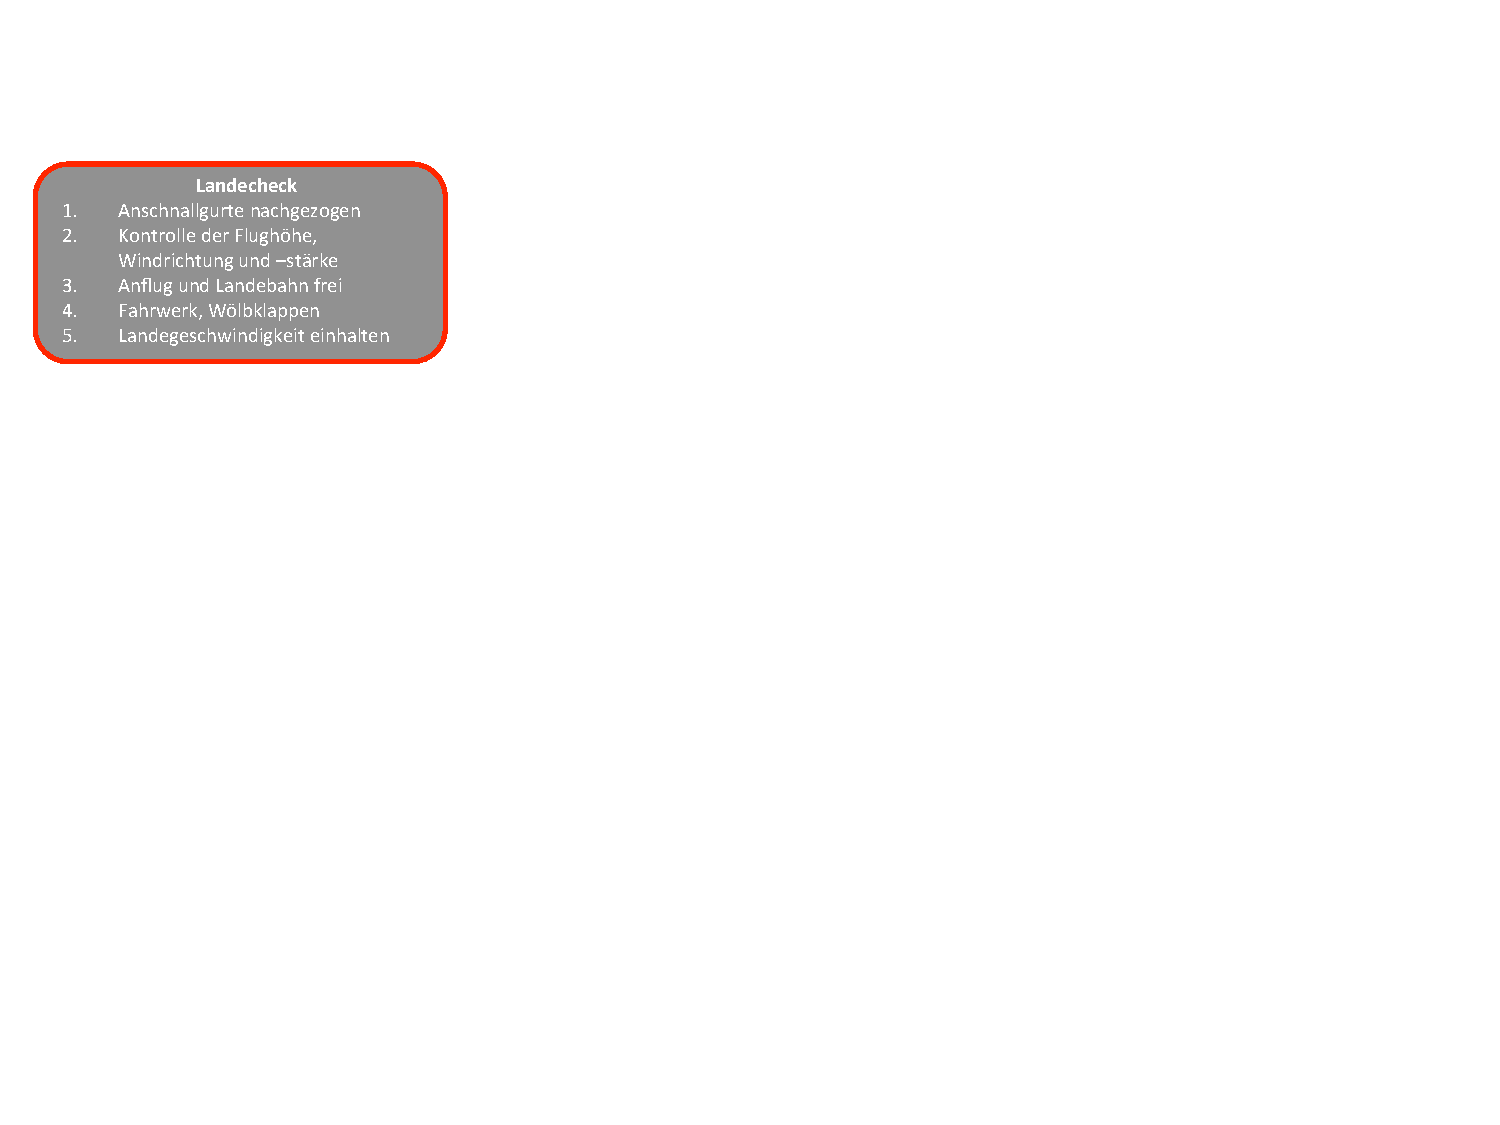
\includegraphics[width=.45\textwidth]{bilder/landecheck.pdf}
\end{center}

Vergewissern Sie sich, dass der \glqq Engine\grqq-Schalter ausgeschaltet ist und der Propeller eingezogen ist.\\

Die normale Anfluggeschwindigkeit für die maximale Masse mit voll ausgefahrenen Bremsklappen und ausgefahrenem Fahrwerk liegt bei $\unit[100]{\frac{km}{h}}$ (gelbes Dreieck auf dem Fahrtmesser).\\
Die Wirkung eines Seitengleitfluges ist gering. Die Wirkung der dreistöckigen Bremsklappen ist mäßig. (Gleitzahl bei ausgefahrenen Bremsklappen ca. $7,2$) \\
Für kurze Landungen über ein Hindernis wird es erfahrenen Piloten empfohlen, schon in größerer Höhe die Fahrt zu reduzieren, da die Wirkung des Bodeneffektes beachtlich ist.\\
Die B13 sollte mit voll gezogenem Höhenruder in 2-Punkt-Lage aufgesetzt werden, Spornradlandungen sind auch problemlos möglich. Nach dem Aufsetzen sollte auf die Wölbklappenstellung $-2$ umgewölbt werden, um die Querruderwirkung bis zum Stillstand aufrecht zu erhalten. Es empfiehlt sich, den Copiloten dabei die Bremsklappen in der gewünschten Stellung festhalten zu lassen, um ein hereinfallen dieser zu verhindern. \\
Die Radbremse wird bei vollem ausfahren der Bremsklappen mitbetätigt und ist gut wirksam.
Das Fahrwerk muss immer ausgefahren werden, da es den Piloten und die Flugzeugstruktur vor starken Landestößen schützt.\\
\newline
\begin{color}{blue}
\large{\underline{Anmerkung}}\\
Aufgrund der Sitzposition sollte die Platzrunde in Richtung des fliegenden Luftfahrzeugführers bevorzugt werden, da die Sichtverhältnisse zur anderen Seite eingeschränkt sind.
\end{color}\\
\newline
\begin{color}{forestgreen}
\large{\underline{Wichtiger Hinweis}}\\
Der Seitengleitflug ist nur wenig wirksam und deshalb als Landehilfe nur bedingt geeignet.
\end{color}\\


\chapter{Flugleistungen}

\deftripstyle{Flughandbuch}[.5pt][.5pt]{\pagemark}{}{\headmark}{Flug- und Betriebshandbuch B13}{}{05.2013}
\pagestyle{Flughandbuch}
\renewcommand*\chapterpagestyle{Flughandbuch}


\section{Einführung}
Der vorliegende Abschnitt enthält anerkannte Werte bezüglich Anzeigefehler der
Fahrtmesseranlage, Überziehgeschwindigkeit und Startleistung sowie zusätzliche
andere Werte und Angaben, die keine Anerkennung durch das LBA benötigen.
Die Daten in den Tabellen wurden durch Erprobungsfluge mit einem Motorsegler
in gutem Zustand unter Zugrundelegung eines durchschnittlichen Pilotenkönnens
ermittelt.

\newpage


\subsection{Nachgewiesene Seitenwindkomponenten}
Noch nicht nachgewiesen.
%\begin{tabular}{l l}
%Windenstart: & ?$\frac{km}{h}$\\
%Flugzeugschlepp: & ?$\frac{km}{h}$\\
%Landung: & ?$\frac{km}{h}$\\
%
%\end{tabular}
\section{Geschwindigkeitspolare}
Die Leistungsvermessung der B13 fand im August 1992 in Aalen-Elchingen statt. Die Flugmasse (Rüstmasse+$180kg$) lag bei $765 kg$, was einer Flächenbelastung von $\frac{G}{S}=396 \frac{N}{m^2}$ entspricht. \\
\newline
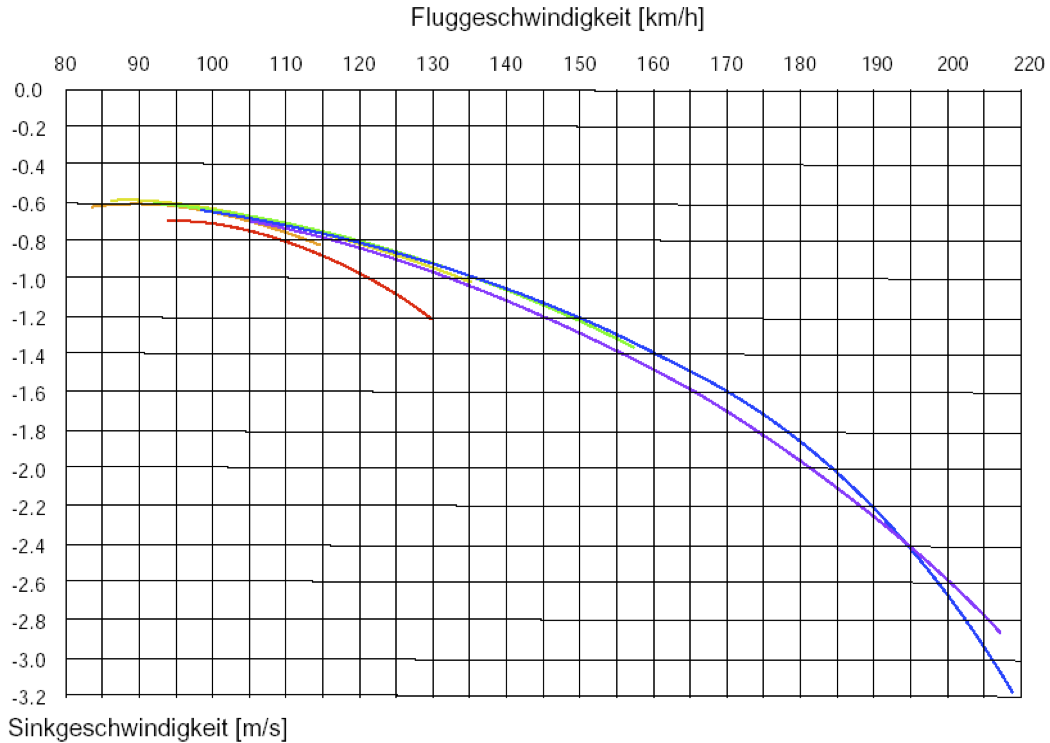
\includegraphics[width=\textwidth]{polare.png}
\newline
\begin{center}
\begin{tabular}{|c|c|c|}
\hline
Wölbklappenstellung & WK-Innen & WK-Außen\\
\hline
\begin{color}{red} L \end{color} & \begin{color}{red} $15,8^{\circ}$ \end{color} & \begin{color}{red} $11,5^{\circ}$ \end{color}\\
\hline
\begin{color}{orange} $+2$ \end{color} & \begin{color}{orange} $10,4^{\circ}$ \end{color} & \begin{color}{orange} $7,5^{\circ}$ \end{color}\\
\hline
\begin{color}{yellow} $+1$ \end{color} & \begin{color}{yellow} $4,5^{\circ}$ \end{color} & \begin{color}{yellow} $3,2^{\circ}$ \end{color}\\
\hline
\begin{color}{cyan} $0$ \end{color} & \begin{color}{cyan} $0^{\circ}$ \end{color} & \begin{color}{cyan} $0^{\circ}$ \end{color}\\
\hline
\begin{color}{blue} $-1$ \end{color} & \begin{color}{blue} $-4,3^{\circ}$ \end{color} & \begin{color}{blue} $-3,2^{\circ}$ \end{color}\\
\hline
\begin{color}{violet} $-2$ \end{color} & \begin{color}{violet} $-9,7^{\circ}$ \end{color} & \begin{color}{violet} $-7,3^{\circ}$ \end{color}\\
\hline

\end{tabular}
\end{center}
\section{Gleitzahlpolare}
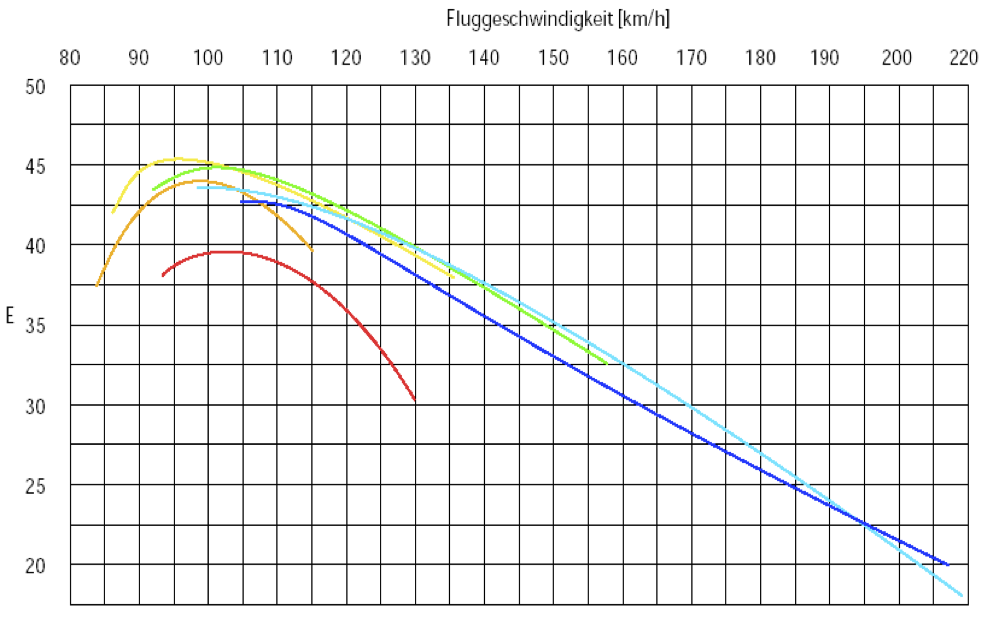
\includegraphics[width=\textwidth]{gzpolare.png}
\newline
\begin{center}
\begin{tabular}{|c|c|c|}
\hline
Wölbklappenstellung & WK-Innen & WK-Außen\\
\hline
\begin{color}{red} L \end{color} & \begin{color}{red} $15,8^{\circ}$ \end{color} & \begin{color}{red} $11,5^{\circ}$ \end{color}\\
\hline
\begin{color}{orange} $+2$ \end{color} & \begin{color}{orange} $10,4^{\circ}$ \end{color} & \begin{color}{orange} $7,5^{\circ}$ \end{color}\\
\hline
\begin{color}{yellow} $+1$ \end{color} & \begin{color}{yellow} $4,5^{\circ}$ \end{color} & \begin{color}{yellow} $3,2^{\circ}$ \end{color}\\
\hline
\begin{color}{cyan} $0$ \end{color} & \begin{color}{cyan} $0^{\circ}$ \end{color} & \begin{color}{cyan} $0^{\circ}$ \end{color}\\
\hline
\begin{color}{blue} $-1$ \end{color} & \begin{color}{blue} $-4,3^{\circ}$ \end{color} & \begin{color}{blue} $-3,2^{\circ}$ \end{color}\\
\hline
\begin{color}{green} $-2$ \end{color} & \begin{color}{green} $-9,7^{\circ}$ \end{color} & \begin{color}{green} $-7,3^{\circ}$ \end{color}\\
\hline

\end{tabular}
\end{center}
\newpage
\section{Leistungsoptimale Wölbklappenbedienung}
Auf Grundlage der Polaren ergeben sich für die verschiedenen Manöver die optimalen Wölbklappenstellungen:\\
\newline
\begin{tabular}{|m{3,5cm}|m{2cm}|m{4cm}|}
\hline
Verwendung & WK-Stellung & Geschwindigkeit [$\frac{km}{h}$]\\
\hline
langsames Kreisen in Ruhiger Thermik & $+2$ & $85$ bis $100$\\
\hline
schnelleres Kreisen in der Thermik, bestes Gleiten, geringstes Sinken & $+1$ & $90$ bis $105$\\
\hline
Gleitflug zwischen Aufwinden & $0$ & $100$ bis $135$\\
\hline
Gleitflug mit erhöhter Geschwindigkeit & $-1$ & $130$ bis $195$\\
\hline
schneller Gleitflug & $-2$ & $190$ bis $220$\\
\hline
\end{tabular}\\
\newline
\newline
Bei Erhöhung der Flächenbelastung und der Schräglage im Kreisflug erhöhen sich auch die Geschwindigkeiten.

\section{Nicht LBA-anerkannte weitere Informationen}
\subsection{Flugleistung im motorgetriebenen Flug}
\subsubsection{Steigrate}

\begin{color}{red}
\large{\underline{Warnung}}\\
Diese Werte sind bisher rechnerisch ermittelt:
\end{color}\\

Die maximale Steigrate kann nur für ca. 14 Minuten bei vollgeladenen Akkupacks erreicht werden, da durch die reduzierte Spannung auch die Steigrate sinkt.

Die durchschnittliche Steigrate hängt von vielen Faktoren ab, vor allem aber von der Abflugmasse.

Der maximale Höhengewinn unter Bedingungen der Standardatmosphare hängt hauptsachlich von der Abflugmasse ab. Für den maximalen Höhengewinn sollte mit einer Leistung von ca. 20kW geflogen werden (nicht maximale Leistung, da das Optimum bei einer geringeren Einstellung liegt).\\ 
Die Steiggeschwindigkeit liegt normalerweise bei 80-85km/h bei positiver Klappenstellung (wie in der Thermik).\\
Der rechnerische ermittelte Wert ist: 1100 m 

\subsubsection{Reiseflug}
Die maximale Reichweite im Reiseflug ist noch nicht ermittelt. 

% noch nicht fertig
\subsubsection{Dienstgipfelhöhe}
Ein Flug in großer Höhe mit einem mit FES ausgestatteten Segelflugzeug ist kein Problem aufgrund von niedrigem Druck. Nach den UN-Transportvorschriften müssen die Zellen, die in den FES Akkupacks verwendet werden acht verschiedene Tests bestehen. Zuerst wird eine Höhensimulation durchgeführt, bei der die Zellen bei einem reduzierten Druck von 11.6kPa (ca. 15.000m) getestet werden.\\

Die tiefen Außentemperaturen von bis zu -20$^\circ$C stellen weder ein Sicherheitsrisiko für
die Akkupacks (die normalerweise wärmer bleiben), noch für andere Komponenten des Antriebssystems dar. Dennoch ist die Leistung der Akkupacks bei tiefen Temperaturen geringer.

\subsubsection{Lärmdaten} 
Die Lärmmesswerte des Motors sind deutlich geringer als die eines vergleichbaren Segelflugzeugs mit Verbrennungsmotor.
Für Hilfstriebwerke gibt es in diesem Rahmen keine Lärmbeschränkungen.\\

Bezüglich des ENL (Engine Noise Level) Signals für Logger:\\
Es wird darauf hingewiesen, dass zur Erkennung des ENL-Signals bei laufendem Motor der Flugdatenlogger im Instrumentenbrett oder vergleichbar nahe an der FES-Einheit angebracht werden muss. Bei einer anderweitigen Positionierung des Loggers im
Cockpit ist ein separater MOP-Sensor wie für andere leise elektrische Motoren anzubringen.
Es sei auf Annex B des IGC Sporting Code verwiesen.

\subsubsection{Elektromagnetische Störungen}
Es konnte kein ungewöhnliches Verhalten der Instrumente durch die Verkabelung die unter dem Instrumentenbrett verlauft (inklusive Magnetkompass) wahrend des Motorbetriebes oder des Anhaltens festgestellt werden.




%\chapter{Masse und Schwerpunktlage}
\section{Einführung}
Dieser Abschnitt enthält den Zuladungsbereich, innerhalb dessen das Segelflugzeug sicher betrieben werden darf.\\
Verfahren zum Wiegen des Segelflugzeuges und eine Beispielrechnung zur Ermittlung der zulässigen Beladegrenzen wird im Anhang aufgeführt.
\section{Definierte Massen, Hebelarme und Schwerpunktlagen}
\textbf{Massen}\\
\begin{tabular}{m{6,5cm} m{3cm}}

Maximale Flugmasse & $m_{max}=800kg$\\
Maximale Masse im Gepäckfach & $m_{G,max}=10kg$\\
Höchstzulässige Masse der nichttragenden Teile einschl. Zuladung & $m_{NT,max}=468kg$\\

\end{tabular}\\
\newline
\newline
\textbf{Zulässige Schwerpunktlagen}\\
\begin{tabular}{m{6,5cm} m{4cm}}
Vorderste Flugmassenschwerpunktlage & $x_{vorn}=245,3mm$\\
Hinterste Flugmassenschwerpunktlage & $x_{hinten}=428,6mm$\\

\end{tabular}\\
\newline
\newline
\textbf{Hebelarme}\\
\begin{tabular}{m{6,5cm} m{3cm}}
Piloten & $x_P=-445mm$\\
Gepäckfach & $x_G=200mm$\\

\end{tabular}\\
\newline
Die Bezugsebene ist die Vorderkante der Wurzelrippe.
\section{Wägebericht}
\begin{tiny}
\begin{tabular}{|m{1,8cm}|m{1,8cm}|m{2cm}|m{1,5cm}|m{1,5cm}|}
\hline
Datum & Leermasse [$kg$] & Leermassen- schwerpunkt [$mm$]  & Maximale Zuladung [$kg$] & Unterschrift\\

\hline

& & & &\\
14.03.12 & 579 & 552,9 & 221 & Hofmann\\
& & & &\\
\hline
& & & &\\
& & & &\\
& & & &\\
\hline
& & & &\\
& & & &\\
& & & &\\
\hline
& & & &\\
& & & &\\
& & & &\\
\hline
& & & &\\
& & & &\\
& & & &\\
\hline

\end{tabular}
\end{tiny}
%\section{Ausrüstungsverzeichnis}
%Stand: 09.03.2012\\
%\begin{tabular}{|l|l|l|l|l|}
%\hline
%Benennung & Baumuster & Hersteller & Einbauort\\
%\hline
%
%
%\end{tabular}
\chapter{Beschreibung d. Motorseglers, seiner Systeme und Anlagen}

\section{Einführung}
Der vorliegende Abschnitt enthält eine Beschreibung des Motorsegelflugzeuges sowie seiner Systeme und Anlagen mit Benutzungshinweisen. 

\section{Bedienorgane}
Jeder Sitz ist ausgestattet mit Steuerknüppel, Seitenruderpedalen, Brems- und Wölbklappenhebel (jeweils links) und Ausklinkknopf (zwischen den Beinen).\\
Haubenverriegelung: Bedienhebel im Instrumentenpilz.\\
Haubennotabwurf: Zusätzlich zum Bedienhebel im Instrumentenpilz den roten Griff dahinter ziehen.\\
Die Bremse ist mit der Bremsklappe gekoppelt und wird im hinteren Bereich der Bremsklappen mit betätigt.\\
Die Trimmung ist in der Mittelkonsole angeordnet. Die Betätigung erfolgt durch Ziehen nach links und verschieben des Hebels (Rastung durch Federkraft).\\
Die Lüftung befindet sich links und rechts neben den Sitzen. Die Betätigung erfolgt durch Entriegeln,  ziehen nach hinten und verriegeln\\


\section{Fahrwerk}
Der Bedienhebel für das Fahrwerk befindet sich in der Mittelkonsole und wird durch umlegen des Hebels betätigt.\\
Beim Einfahren des Fahrwerkes empfiehlt es sich, den Hebel in einem Zug nach hinten durch zu ziehen.\\
Zum Ausfahren des Fahrwerkes den Hebel aus der Verknieung drücken, Hebel dann langsam nach vorn führen um ein durchschlagen zu verhindern und in vordere Verknieung drücken.\\
Die hydraulische Doppelscheibenbremse wird mit vollständigem Ausfahren der Bremsklappen mitbetätigt und ist gut wirksam.


\section{Instrumentierung}
Im Instrumentenpilz (Abb. 6.1) sind die Instrumente zur Flugüberwachung (Fahrtmesser mit Meßbereich mindestens $50 \frac{km}{h}$ bis $300 \frac{km}{h}$ ,Höhenmesser, Variometer), Funksprechgeräte und Navigationsgeräte angeordnet.

\begin{figure}[ht]
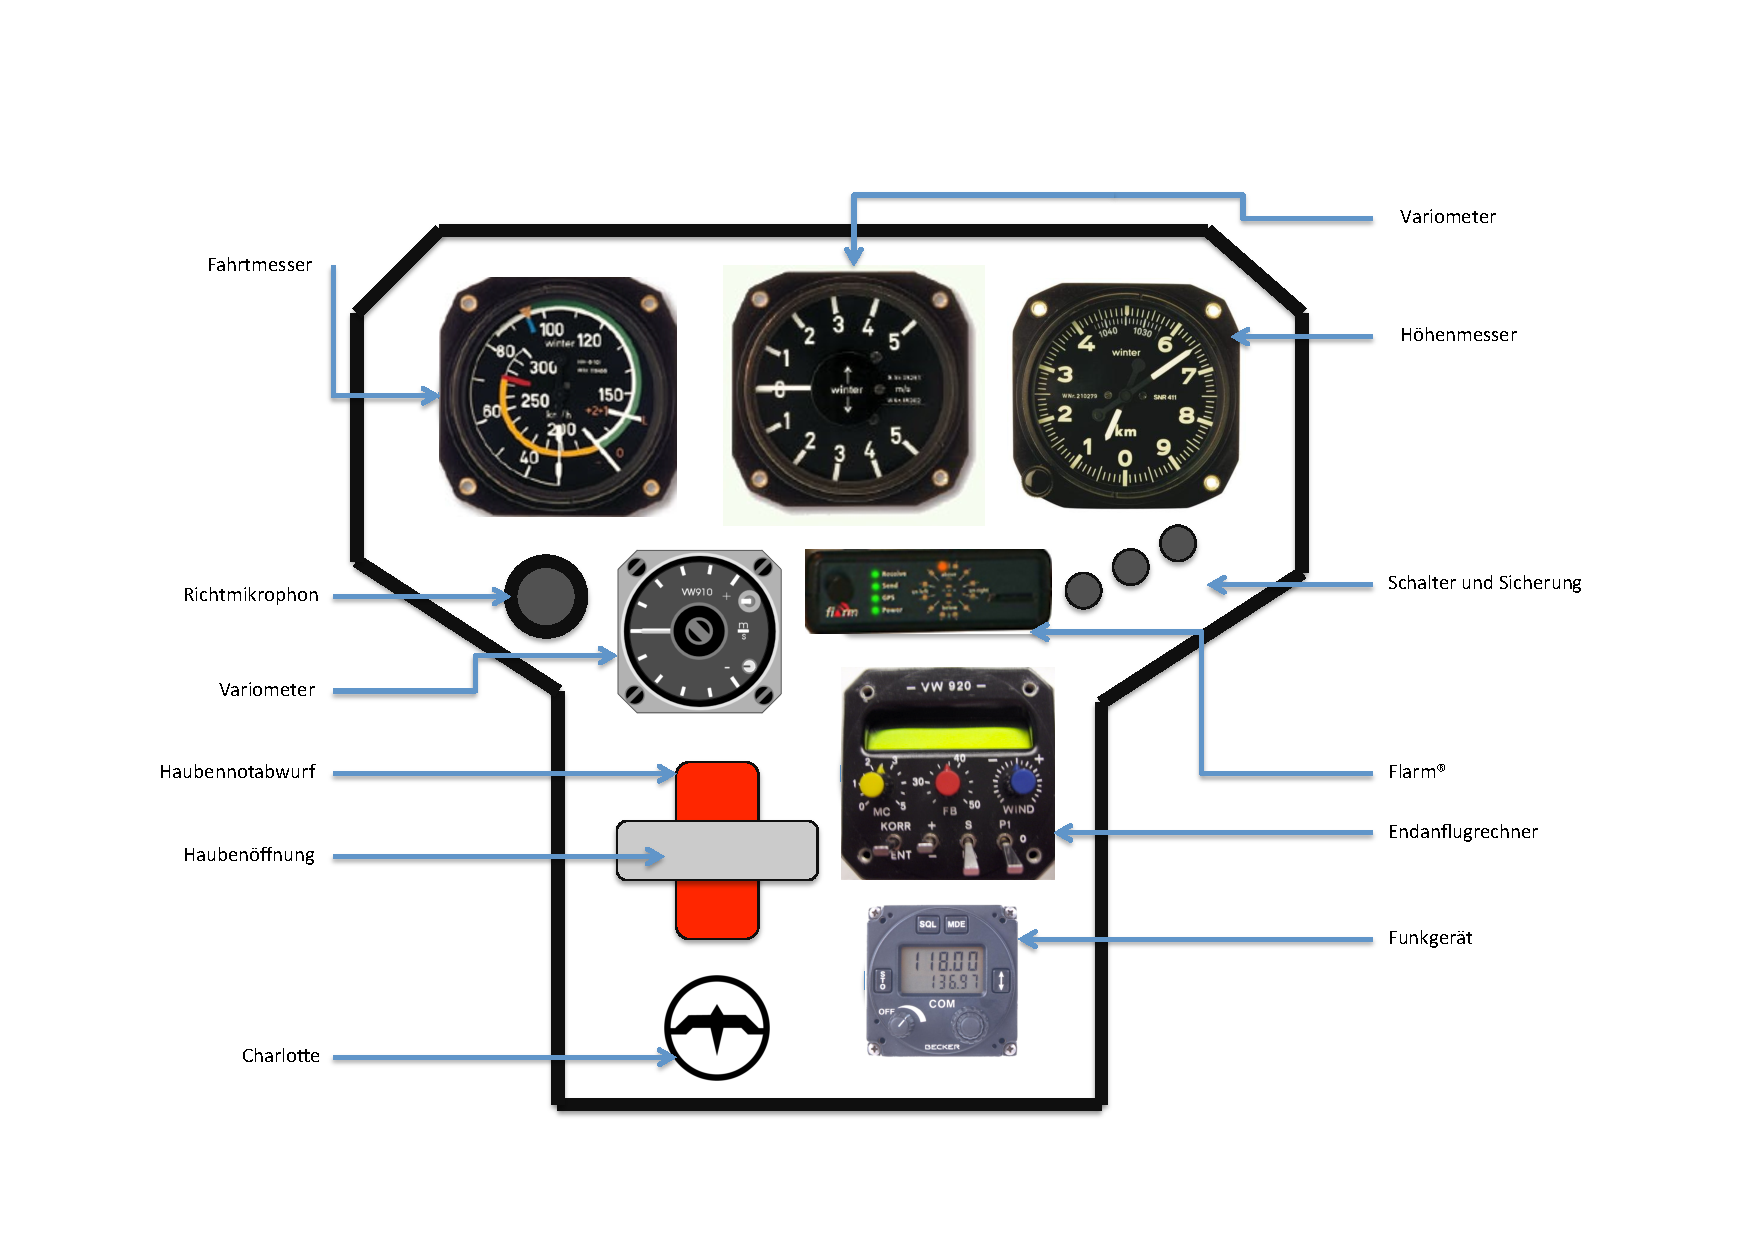
\includegraphics[angle=90,width=\textwidth]{bilder/instrumentenpilz.pdf}
\caption{Instrumentenpilz}
\end{figure}

\section{Bremsklappen}
Doppelstöckige Schempp-Hirth Bremsklappen auf der Oberseite des Innentragflügels. Der Antrieb mit Verknieung ist im Mittelrumpf angeordnet.

\section{Gepäckraum}
Das Gepäckfach befindet sich hinter dem rechten Piloten und hat eine maximale Zuladung von $10kg$.

\newpage
\section{Triebwerksanlage}
nicht eingebaut

\newpage
\section{Faltpropeller}
nicht eingebaut
\chapter{Pflege und Instandhaltung}
\section{Einführung}
In diesem Abschnitt werden empfohlene Verfahren zur korrekten Handhabung des Flugzeugs am Boden sowie zur Instandhaltung beschrieben. Darüber hinaus werden bestimmte Prüf- und Wartungsbestimmungen aufgezeigt, die eingehalten werden sollten, wenn der Motorsegler die einem neuen Gerät entsprechende Leistung und Zuverlässigkeit erbringen soll. Es ist ratsam, einen Schmierplan einzuhalten und unter Zugrundelegung der besonderen klimatischen sowie sonstigen Betriebsbedingungen vorbeugende Wartungsmaßnahmen durchzuführen.

%\section{Prüfintervalle}
%Es liegt noch kein Wartungshandbuch für die B13 vor. \\
%\newline
%Generell muss die B13 regelmäßig einmal pro Jahr und nach größeren Reparaturen gewartet und nachgeprüft werden. \\
%\newline
%Dabei sollten mindestens folgende Wartungen durchgeführt werden:
%\begin{itemize}
%\item Gesamtes Flugzeug auf Risse, Löcher und Beulen untersuchen
%\item Anschlussbeschläge auf einwandfreien Zustand (Spiel, Riefen, Korrosion) kontrollieren 
%\item Metallteile (besonders der Steuerungsanlagen) auf Korrosion überprüfen, ggf. neu konservieren
%\item Anschlüsse von Flügel und Leitwerke auf Spiel kontrollieren
%\item Steuerung (besonders Bremsklappen) sind einer Funktionskontrolle zu unterziehen
%\item Ruderausschläge und Anschlagpunkte der Steuerung nachprüfen
%\item Fahrwerk und Schwerpunktkupplung kontrollieren 
%\item Druckentnahmestellen der Druckanlagen auf Sauberkeit und die Leitungen auf Dichtigkeit überprüfen
%\item Zustand und ordnungsgemäße Funktion aller Instrumente, Geräte und Ausrüstungsteile ist zu überprüfen
%\end{itemize}
%
%Zusätzlich sollten vor jedem Aufrüsten alle Anschlussbolzen und –buchsen sowie Leitwerks- und Flügelanschlüsse gereinigt und gefettet werden. \\
%\newline
%Da noch kein Schmierplan für die B13 vorliegt, sind die entsprechenden Lager des Öfteren zu kontrollieren und bei Bedarf nachzuschmieren. \\

\section{Änderungen oder Reparaturen}
Die verantwortliche Luftfahrtbehörde ist unbedingt \textbf{vor} jeder Änderung an dem Motorsegler zu unterrichten, um sicherzustellen, dass die Lufttüchtigkeit des Motorseglers nicht gefährdet wird. Erst nach Genehmigung der Änderungen von der Luftfahrtbehörde dürfen diese durchgeführt werden. \\
\newline
Größere Reparaturen sollten nur von fachkundigem Personal mit entsprechender Berechtigung durchgeführt werden. 
\newpage
\section{Handhabung am Boden/Straßentransport}

\subsection{Ziehen/Schieben}
Das Schleppen am Boden sollte über ein Seil mit einem Doppelring, welcher in der Schwerpunktkupplung eingehängt wird, erfolgen. Es sollte neben einer Person an der Fläche noch eine zweite Person in Nähe des Ausklinkknopfes den Schlepp begleiten. \\
\newline
Weiterhin ist für den Transport am Boden unbedingt der dafür vorgesehene Spornkuller zu verwenden. Die B13 hat zwei Spornkuller. Der größere Kuller enthält noch zusätzliche Auflageflächen zur Befestigung der Außenflächen während des Straßentransportes im Anhänger. Dieser Kuller eignet sich nicht für das Ziehen und Schieben am Boden. \\
Auf ausreicheden Luftdruck und festen Sitz ist bei dem normalen Kuller aufgrund der hohen Spornlast unbedingt zu achten.\\
\newline
\begin{color}{forestgreen}
\large{\underline{Wichtiger Hinweis}}\\
Zur Befestigung des Spornkullers sollte nicht auf die Nase gedrückt werden, da die Nase nur eine Abdeckung ist und keine tragende Wirkung hat.
\end{color}\\
\newline
Das Bewegen der B13 am Boden ohne Kuller sollte nur in Ausnahmefällen geschehen und ohne große Krafteinleitungen, die eine Bewegung um die Hochachse erzeugen, durchgeführt werden, damit der Sporn (insbesondere das Spornrad) und die Leitwerke nicht zu stark belastet werden.\\
\newline
Die Haube muss dabei in jedem Fall verriegelt werden. Es wird empfohlen, den vorderen Haubenspalt mit einem Mylarband, welches am Haubenrahmen befestigt wird, abzudichten, da es sonst während des Fluges zu unangenehmen Geräuschen kommen kann. 

\subsection{Abstellen und Lagern}
Die B13 sollte nur in gut belüfteten Räumen und Transportanhängern abgestellt und transportiert werden. Ein längeres Abstellen unter starker Sonneneinstrahlung oder Feuchtigkeit sollte möglichst vermieden werden, da es die Oberfläche deutlich schneller altern lässt.\\
\newline
Die Oberfläche (mindestens die Haube) sollte noch zusätzlich durch weiche, saubere Bezüge abgedeckt werden. 

\subsection{Vorbereitung auf den Straßentransport}
Der Transport der B13 erfolgt in dem dafür vorgesehenen Transportanhänger. Vor dem Transport sollten unbedingt alle lockeren Gegenstände aus dem Cockpit entfernt und die nun losen Steuerstangen im Rumpf mit den dafür vorgesehenen Schonern bezogen werden. \\
\newline
Durch ihren breiten Rumpf wurde ein Befestigungssystem für die Außenflächen auf dem Rumpf vorgesehen. Um ein Loslösen der Außenflächen von der Halterung zu verhindern, ist auf eine vollständige Sicherung der Verschlüsse für die Halterungen hinter dem Cockpit und am Spornkuller zu achten. Auch der Rumpf und die Innenflächen sollten richtig in ihre Halterungen geschoben und anschließend gesichert werden. \\
\newline
Generell ist auf eine spannungsfreie Lagerung aller Einzelteile zu achten, da sich gerade bei hohen Temperaturen (wie sie in Transportanhängern auftreten können)  die einzelnen Flugzeugteile verziehen könnten. 

\section{Reinigung und Pflege}
Der Reinigung der Plexiglashaube sollte besondere Aufmerksamkeit geschenkt werden, da sie die freie Sicht der Piloten gewährleistet. Es ist unbedingt darauf zu achten, dass zum Säubern der Haube nur reichlich klares, sauberes Wasser und ein reines Ledertuch verwendet wird. Es sollte niemals trocken auf der Plexiglashaube gerieben werden. \\
\newline
Falls vorhanden, wird der Einsatz spezieller Reinigungsmittel für Plexiglashauben (z.B. Plexiklar) empfohlen. \\
\newline
Die Oberfläche der B13 sollte nach jedem Flugbetrieb mit einem weichen sauberen Schwamm und viel klarem Wasser gereinigt werden. Zum Trocknen wird ein sauberes Ledertuch verwendet. \\
\newline
Klebebandreste können mit ein wenig Silikonentferner entfernt werden. Es sollte kein Aceton oder silikonhaltige Pflegemittel angewandt werden, da es die Lackschicht des Flugzeuges stark angreift oder den Aufwand bei Lackreparaturen deutlich erhöhen könnte. Weiterhin sollten Poliermittel und flüssiges Wachs zur Pflege der Oberfläche angewandt werden. \\
\newline
\begin{color}{forestgreen}
\large{\underline{Wichtiger Hinweis}}\\
Es ist unbedingt darauf zu achten, dass das Flugzeug vor Nässe geschützt wird. 	Eingedrungenes Wasser sollte schnellst möglichst entfernt werden. Dazu muss die B13 trocken gelagert und die abgerüsteten Flugzeugteile  öfters gewendet 	werden. 
\end{color}\\
\newline

Die Schwerpunktkupplung und das Hauptrad sind durch ihren Einbauort starken Verschmutzungen ausgesetzt (besonders nach Außenlandungen). Sie sollten daher laufend auf Verschmutzungen untersucht, gereinigt und geschmiert werden. 
%\input{kapitel9.tex}
%
\addcontentsline{toc}{chapter}{Anhang} 
\begin{appendix}
das ist der anhang
\end{appendix}
%\textbf{Betriebshandbuch}

%\begin{thebibliography}{breitestes Label}
%\bibitem{Aero} Prof. Dr.-Ing. W. Nitsche, {\sl - Gasdynamik I Skript -},
%Sommersemester 2010
%%\bibitem{Versuchsanlagen} Prof. Dr.-Ing. W. Nitsche und Dr.-Ing. A. Brunn, {\sl - 	Strömungsmesstechnik-},
%%2006, 2. Auflage
%\bibitem{windkanal} http://aero.ilr.tu-berlin.de/bilder/logo.gif, 
%28.06.2011
%\end{thebibliography}

\appendix
%\section{MatlabCode - Aufgabe 1}

\end{document} 







